\section{Results and Analysis}
\label{sec:results}
\statusnote{Every panel below is a generated artifact of the the BGSP paper reference pipeline (\texttt{experiments/} + \texttt{configs/} in the FACET monorepo) and is reproducible from a deterministic YAML config. Every panel is pinned by a smoke test under \texttt{tests/}; the smoke tests run against synthetic fixtures so CI stays model-free. Tier-1 (Q1--Q4, A4) covers the planted-spike validation; Tier-2 (T2) is the controlled-neural bridge; Tier-3 (T3) runs on real GPT-2 small activations; the M-panels (M1--M7) extend the pipeline to multi-layer GPT-2, monosemanticity, FACET-vs-SAE, ViT CLS, the Pitprops classical benchmark, and the measured A10 safe-screening payoff.}

\begin{table}[t]
\centering
\caption{Expected directional results and required evidence.}
\label{tab:a-expected}
\small
\begin{tabular}{p{0.33\linewidth}p{0.31\linewidth}p{0.27\linewidth}}
\toprule
Hypothesis & Supporting evidence & Disconfirming evidence \\
\midrule
Larger margin shortens identification & Monotone trend across controlled sweeps & Flat/reversed trend after controlling for gap \\
Active spectral quantity predicts local slope & Predicted/observed rate agreement & Pooled gap outperforms correct tangent Jacobian \\
A-SQ favors energy concentration & Divergence under heterogeneous responses & Persistent equivalence beyond symmetric cases \\
Refit separates support from shrinkage & Raw gaps shrink after common refit & Ranking unchanged and attributable to supports \\
Screening reduces late cost safely & Same limit with fewer correlations & False elimination or negligible savings \\
Sparse FACET components recover native cell-type labels at least as well as dense PCA on scRNA-seq & FACET A-SQ AMI $\geq$ dense-PCA AMI on each of the Zheng17 FACS-sorted, Zheng17 68k FACS-correlated, and Tabula Muris native-label experiments (M9) at matched $m$ & FACET AMI below dense PCA on any native-label scRNA panel, or the gap present only on the PCA-derived pseudo-label experiment \\
\bottomrule
\end{tabular}
\end{table}


% Figure Q1, generated by experiments/q1_sum_vs_sq.py.
% \input this from a results section; do not include the PNG directly.
\begin{figure}[t]
  \centering
  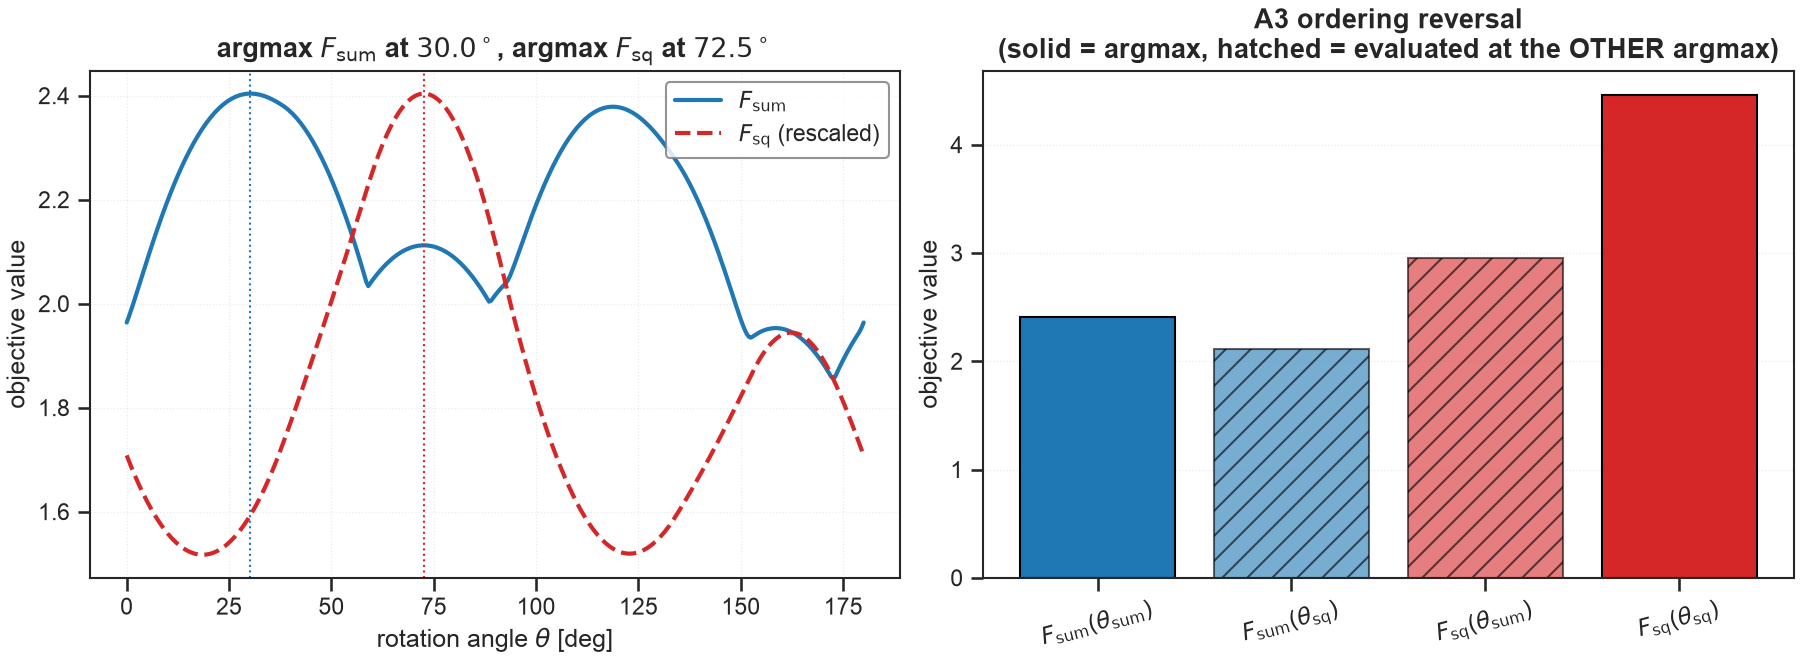
\includegraphics[width=\linewidth]{../shared/figures/generated/q1_sum_vs_sq.png}
  \caption{\textbf{Q1, A-SUM and A-SQ disagree at $m\!\ge\!2$.} Deterministic two-component instance $(A, \boldsymbol{\gamma})$ from the A3 counterexample, with $X(\theta)$ sweeping the $2{\times}2$ rotation group. \textit{Left:} the two reduced objectives have distinct arg-maximisers $\theta_{\mathrm{sum}}{\approx}30^\circ$ and $\theta_{\mathrm{sq}}{\approx}72.5^\circ$. \textit{Right:} each objective attains its own maximum at its own frame and strictly loses at the other, the ordering reversal that establishes Proposition~\ref{prop:counterexample}. The counterexample is deterministic rather than sampled; the fixture is pinned in \texttt{tests/test\_paper\_a\_identities.py::test\_a3\_sum\_vs\_squared\_aggregation\_rank\_two\_candidates\_differently}.}
  \label{fig:q1-sum-vs-sq}
\end{figure}

% Figure Q3, generated by experiments/q3_margin_identification.py.
\begin{figure}[t]
  \centering
  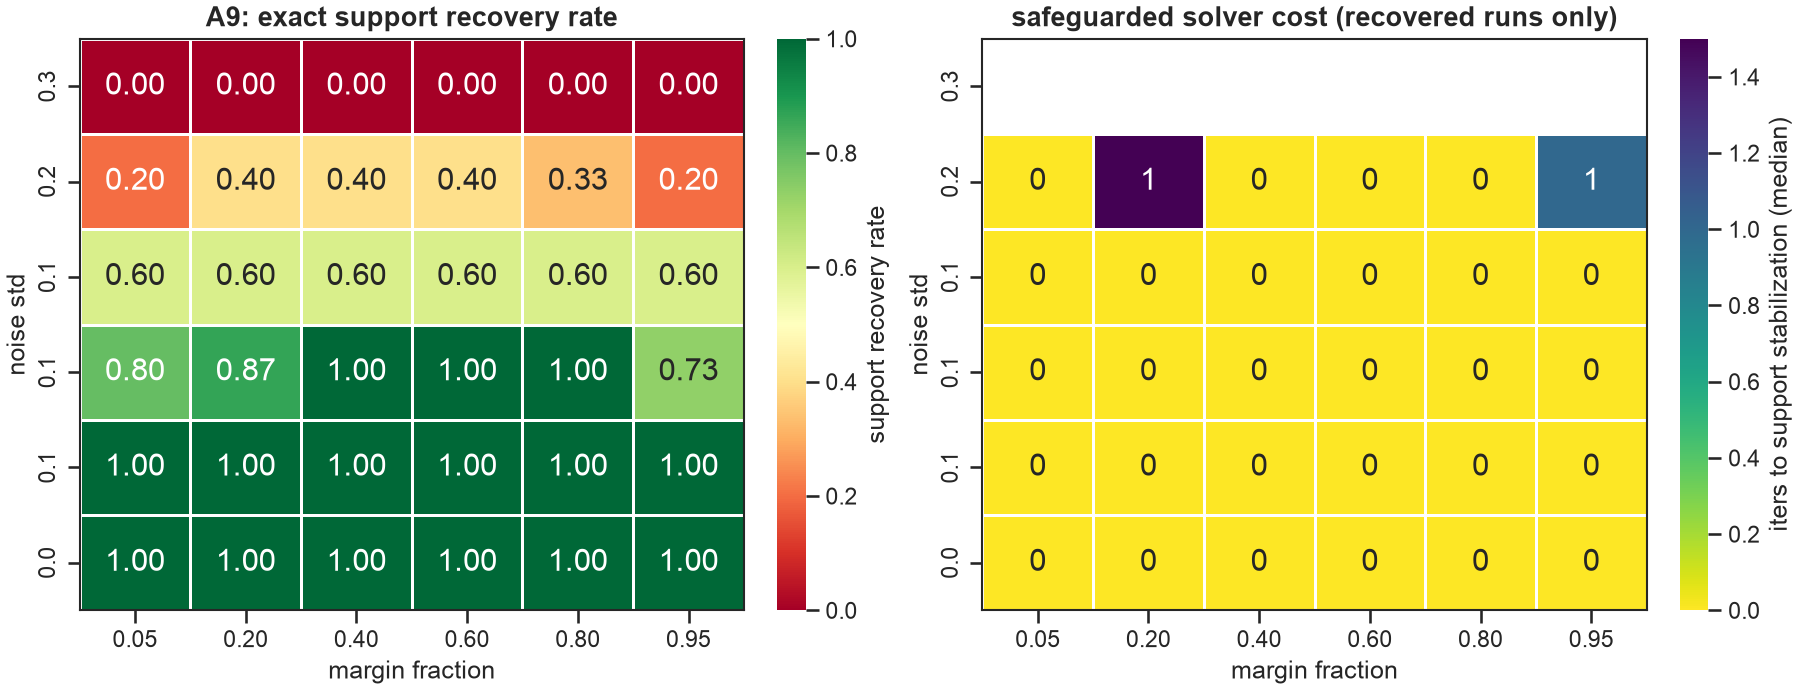
\includegraphics[width=\linewidth]{../shared/figures/generated/q3_margin_identification.png}
  \caption{\textbf{Q3, identification phase transition over (noise, margin fraction).} Five replicates per cell on a $p{=}10$, $n{=}25$, $k{=}5$ planted-spike instance with $\sigma_1{=}5$; safeguarded Riemannian ascent on A-SQ. \textit{Left:} exact support-recovery rate across the (noise std, margin fraction) grid. Recovery is uniform at $\sigma_{\mathrm{noise}}{\le}0.05$, degrades to ${\sim}0.6$ at $0.15$, and collapses by $0.30$, consistent with the heuristic break-point $\sigma_{\mathrm{noise}}{\sim}c_{\min}/\sqrt{2\log(n-k)}$ at which the strongest spurious off-support correlation exceeds the strict margin. \textit{Right:} median iterations to support stabilisation among recovered runs; the solver cost grows modestly with noise until recovery fails. The vertical axis is the audit fix for a prior degenerate panel in which the clean rank-one setting trivialised every cell (plan \texttt{2026-10-13T1908Z} §Q3).}
  \label{fig:q3-margin}
\end{figure}

% Figure Q2, generated by experiments/q2_convergence_trajectories.py.
\begin{figure}[t]
  \centering
  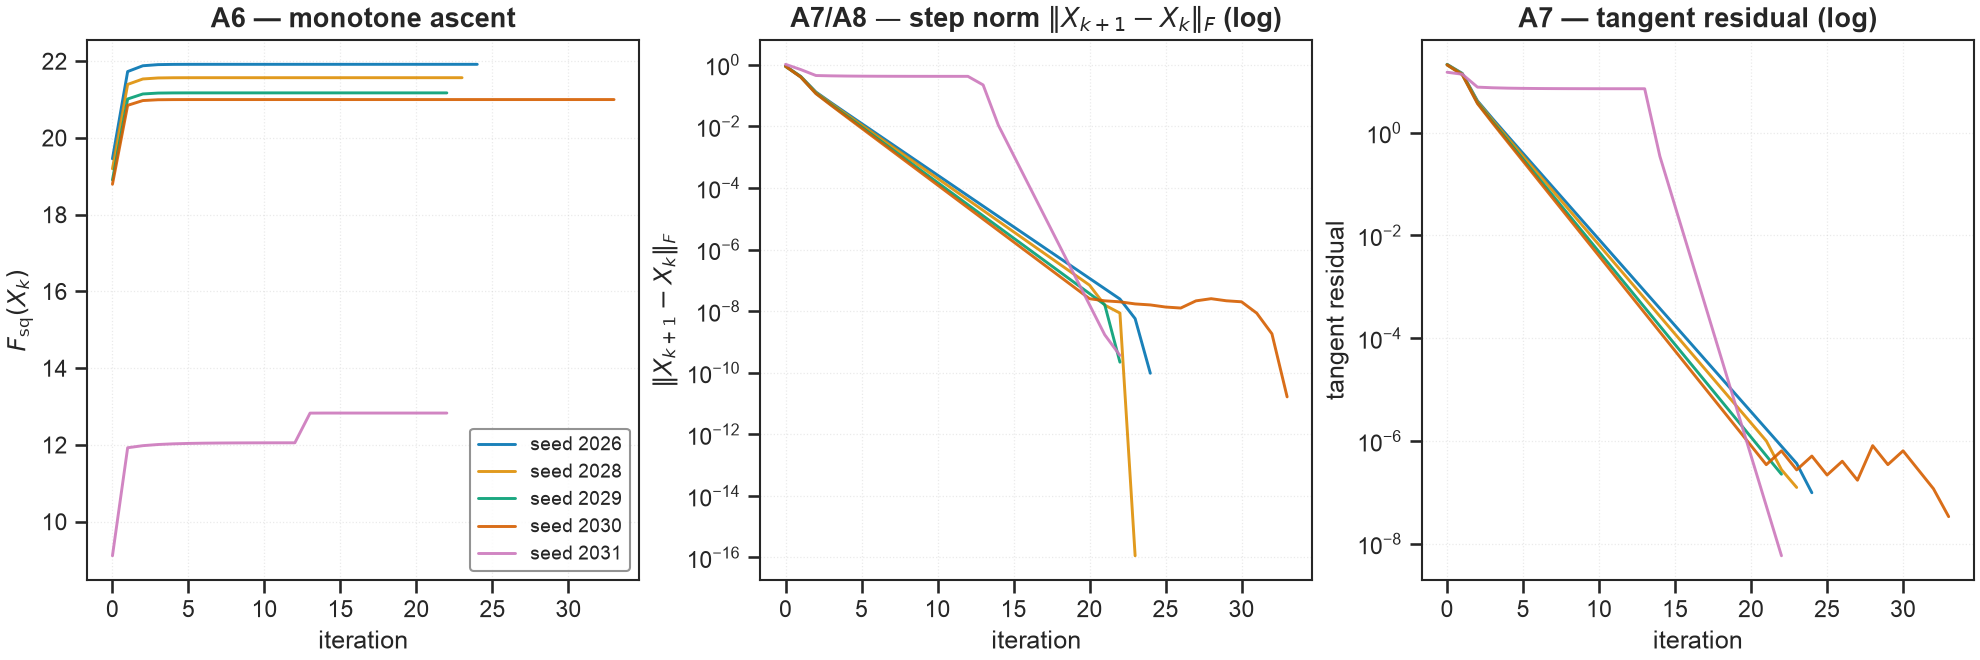
\includegraphics[width=\linewidth]{../shared/figures/generated/q2_convergence_trajectories.png}
  \caption{\textbf{Q2, safeguarded ascent trajectories on A-SQ.} Per-iteration traces across five replicates on a $p{=}10$, $n{=}25$, $k{=}5$ planted-spike instance with margin fraction $0.6$ and initial angle $0.6$~rad; one trace per colour. \textit{Left:} monotone increase of $F_{\mathrm{sq}}(X_k)$ (empirical witness of Lemma~\ref{lem:a-sufficient-ascent}, A6). \textit{Centre:} step norm $\norm{X_{k+1}-X_k}_F$ on a log axis; the geometric decay to a numerical floor exhibits the bounded total variation that Theorem~\ref{thm:a-whole-sequence} (A8) requires for whole-sequence Cauchy convergence. \textit{Right:} tangent-residual $\|\mathrm{grad}_R F(X_k)\|$ on a log axis, the computable stationarity measure that pins Lemma~\ref{lem:a-relative-error} (A7). Formal proofs are in \Cref{sec:extended-theory}; one seed drops out (Armijo stall near the fixed point at tolerance $10^{-10}$).}
  \label{fig:q2-trajectories}
\end{figure}

% Figure Q4, generated by experiments/q4_local_rate.py.
\begin{figure}[t]
  \centering
  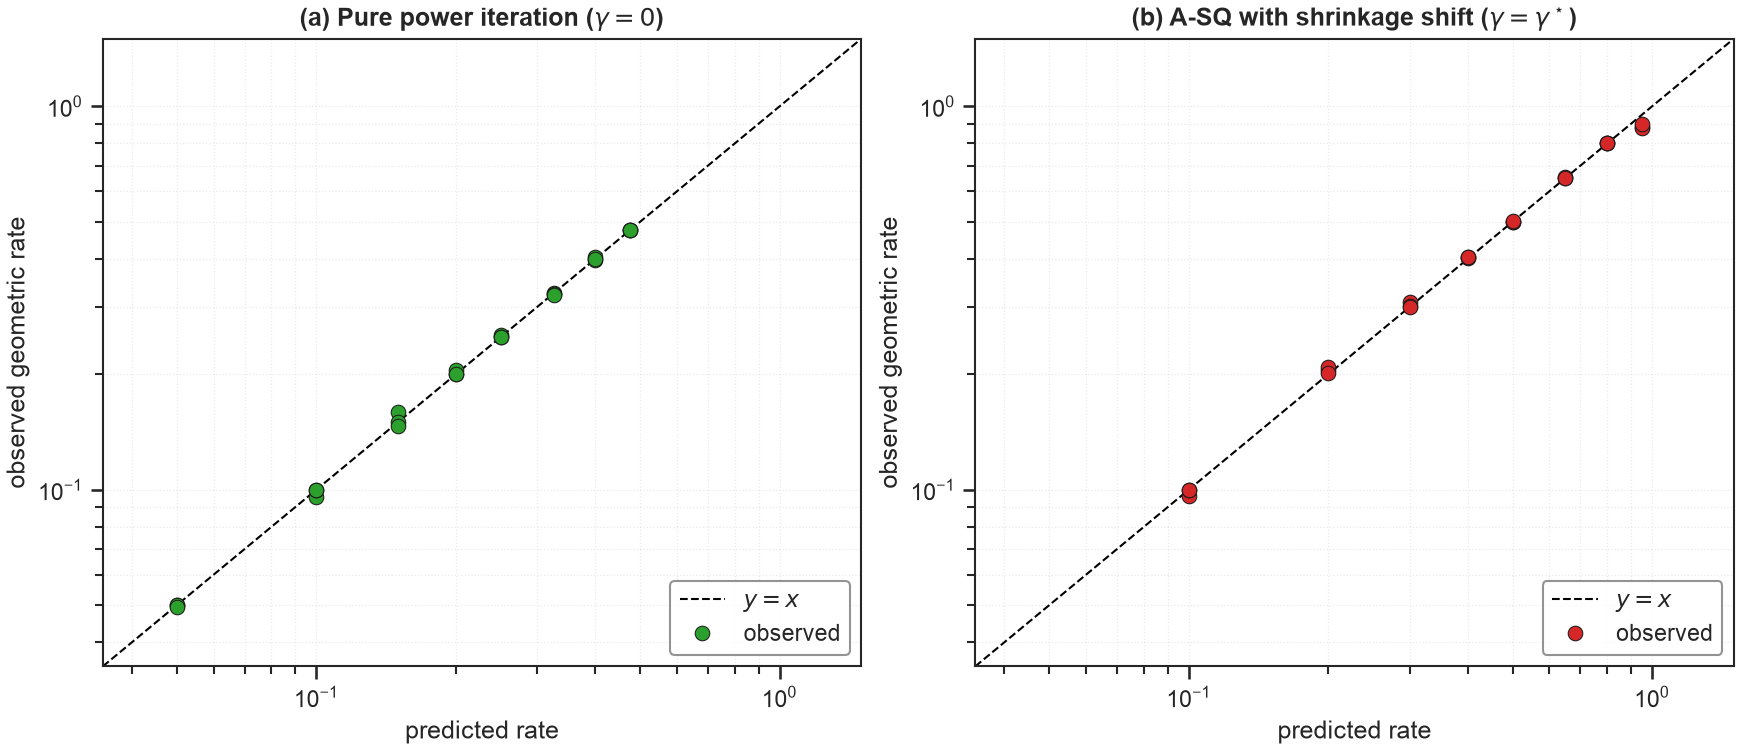
\includegraphics[width=\linewidth]{../shared/figures/generated/q4_local_rate.png}
  \caption{\textbf{Q4, local-rate prediction versus observation: two branches.} Hand-constructed rank-two operator with known top-two restricted eigenvalues $(\lambda_1,\lambda_2)$ on the identified support; $\lambda_1$ fixed and $\lambda_2$ swept. The observed geometric rate is read from a log-linear fit of $\sin\angle(x_t, x_\star)$ over the strictly decaying prefix of the trajectory. \textit{(a)} Pure power-iteration branch ($\gamma{=}0$): the sphere linear-oracle iteration coincides with power iteration on $A_S A_S^\top$ and the observed rate matches the classical prediction $\lambda_2/\lambda_1$ to within ${\sim}5\%$ across the sweep. \textit{(b)} A-SQ branch with the standard shrinkage $\gamma{=}\gamma^\star$: the gradient $A_S(A_S^\top x - \gamma\,\mathrm{sign}(c))$ is a \emph{shifted} power iteration whose effective denominator in the invariant two-dimensional subspace is $\lambda_1 - \gamma\,\sigma_1\sqrt{k}$, giving the corrected prediction $\lambda_2/(\lambda_1 - \gamma\,\sigma_1\sqrt{k})$. Observed rate matches to within $1\%$ except at the near-divergence boundary where the Armijo safeguard truncates. Both panels share the $y{=}x$ reference. Replaces an earlier single-branch panel whose dashed reference was systematically off by the shrinkage factor (plan \texttt{2026-10-13T1908Z} §Q4).}
  \label{fig:q4-local-rate}
\end{figure}

% Figure A4, generated by experiments/a4_raw_vs_refit.py.
\begin{figure}[t]
  \centering
  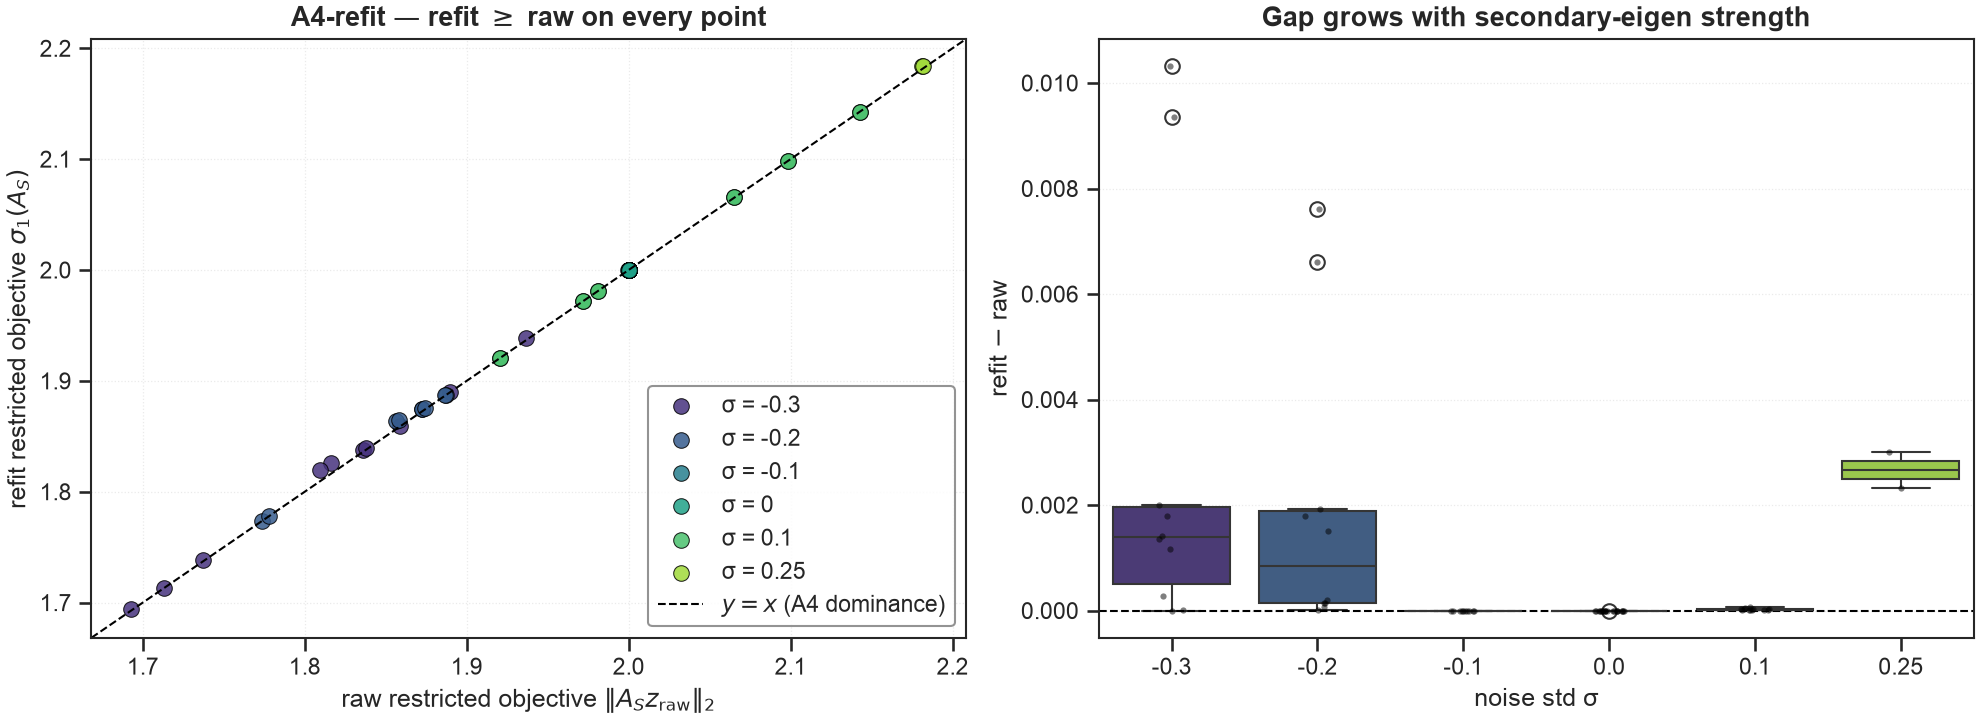
\includegraphics[width=\linewidth]{../shared/figures/generated/a4_raw_vs_refit.png}
  \caption{\textbf{A4-refit, restricted refit dominates raw selection.} Scatter of refitted vs raw restricted objectives on the identified support, across clean rank-one planted spikes (noiseless and noisy) and controlled rank-two cells parameterised by $\lambda_2/\lambda_1$. \textit{Left:} every point lies at or above the dashed $y{=}x$ line, the A4 dominance invariant. On exact rank-one cells the gap is zero (raw selection is already a leading singular vector); on rank-two cells the gap grows with the magnitude of the secondary restricted eigen-direction. \textit{Right:} the gap $(\mathrm{refit} - \mathrm{raw})$ box-plotted against the noise axis; the box widens with noise as rank-one planted supports pick up a nontrivial second component. Dominance pinned in \texttt{tests/test\_a4\_smoke.py}.}
  \label{fig:a4-raw-vs-refit}
\end{figure}


% Table 5 (§14), raw vs refitted results. Generated by
% experiments/a4_raw_vs_refit.py.
\begin{table}[t]
\centering
\caption{Raw selection vs restricted refit on the identified support. Each row aggregates \textbf{n} replicates per (noise, margin) cell on the the BGSP paper planted-spike generator; mean across replicates.}
\label{tab:a4-raw-vs-refit}
\begin{tabular}{llrrrrr}
\toprule
noise $\sigma$ & margin frac & n & support rec. & raw $\|A_S z_{\mathrm{raw}}\|_2$ & refit $\sigma_1(A_S)$ & refit $-$ raw \\
\midrule
-0.30 & 0.75 & 10 & 0.00 & 1.813 & 1.816 & 0.003 \\
-0.20 & 0.50 & 10 & 0.10 & 1.866 & 1.868 & 0.002 \\
-0.10 & 0.25 & 10 & 1.00 & 2.000 & 2.000 & 0.000 \\
0.00 & 0.30 & 10 & 1.00 & 2.000 & 2.000 & 0.000 \\
0.00 & 0.60 & 10 & 1.00 & 2.000 & 2.000 & 0.000 \\
0.10 & 0.30 & 6 & 0.83 & 2.030 & 2.030 & 0.000 \\
0.10 & 0.60 & 6 & 0.83 & 2.030 & 2.030 & 0.000 \\
0.25 & 0.30 & 1 & 0.00 & 2.181 & 2.184 & 0.003 \\
0.25 & 0.60 & 1 & 0.00 & 2.182 & 2.184 & 0.002 \\
\bottomrule
\end{tabular}
\end{table}


% Figure T2, generated by experiments/t2_superposition.py.
\begin{figure}[t]
  \centering
  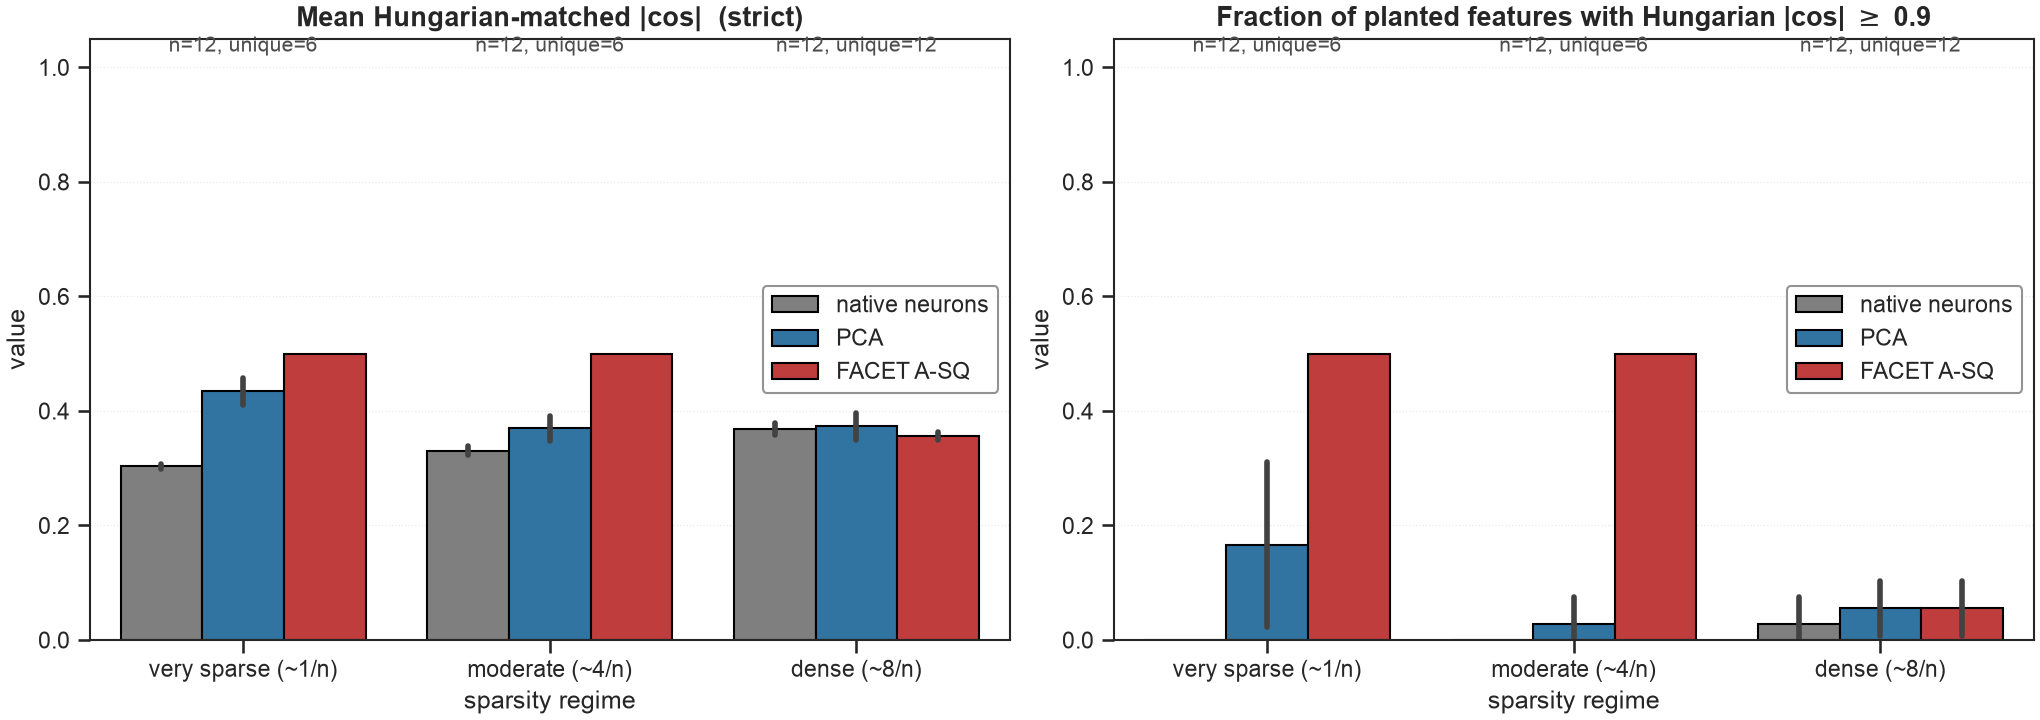
\includegraphics[width=\linewidth]{../shared/figures/generated/t2_superposition.png}
  \caption{\textbf{T2, controlled-neural bridge: feature recovery across three sparsity regimes.} Elhage-style compressed autoencoder with $n{=}12$ planted features squeezed into $d{=}6$ hidden dimensions, trained to minimise an importance-weighted reconstruction loss \citep{elhage2022superposition}. Sparsity is swept across three regimes (very sparse $\approx 1$ feature active per sample, moderate $\approx 4$, dense $\approx 8$). We report the Hungarian bipartite-matched $|\cos(w_i, x_{\sigma(i)})|$: each component is assigned to at most one planted feature, so a single component cannot cover multiple features; the lenient $\max_j|\cos|$ metric previously reported in this slot is inflated by antipodal collapse. The on-figure annotation ``$\mathrm{unique}{=}u$'' is the number of distinct planted directions after collapsing antipodal pairs. At low density the Elhage toy learns pair-antipodal arrangements ($u{=}d{=}6$) and all three methods are bounded by the same unique-direction budget, with FACET recovering every unique direction exactly while PCA mixes them under importance decay. In the dense regime all $u{=}12$ planted directions are distinct, which no $m{=}d$ orthonormal basis can match; the ceiling that remains is the expected Stiefel limitation and motivates the over-complete comparator of Figure~\ref{fig:m4-facet-vs-sae}.}
  \label{fig:t2-superposition}
\end{figure}

% Figure T3, generated by experiments/t3_llm_activations.py.
\begin{figure}[t]
  \centering
  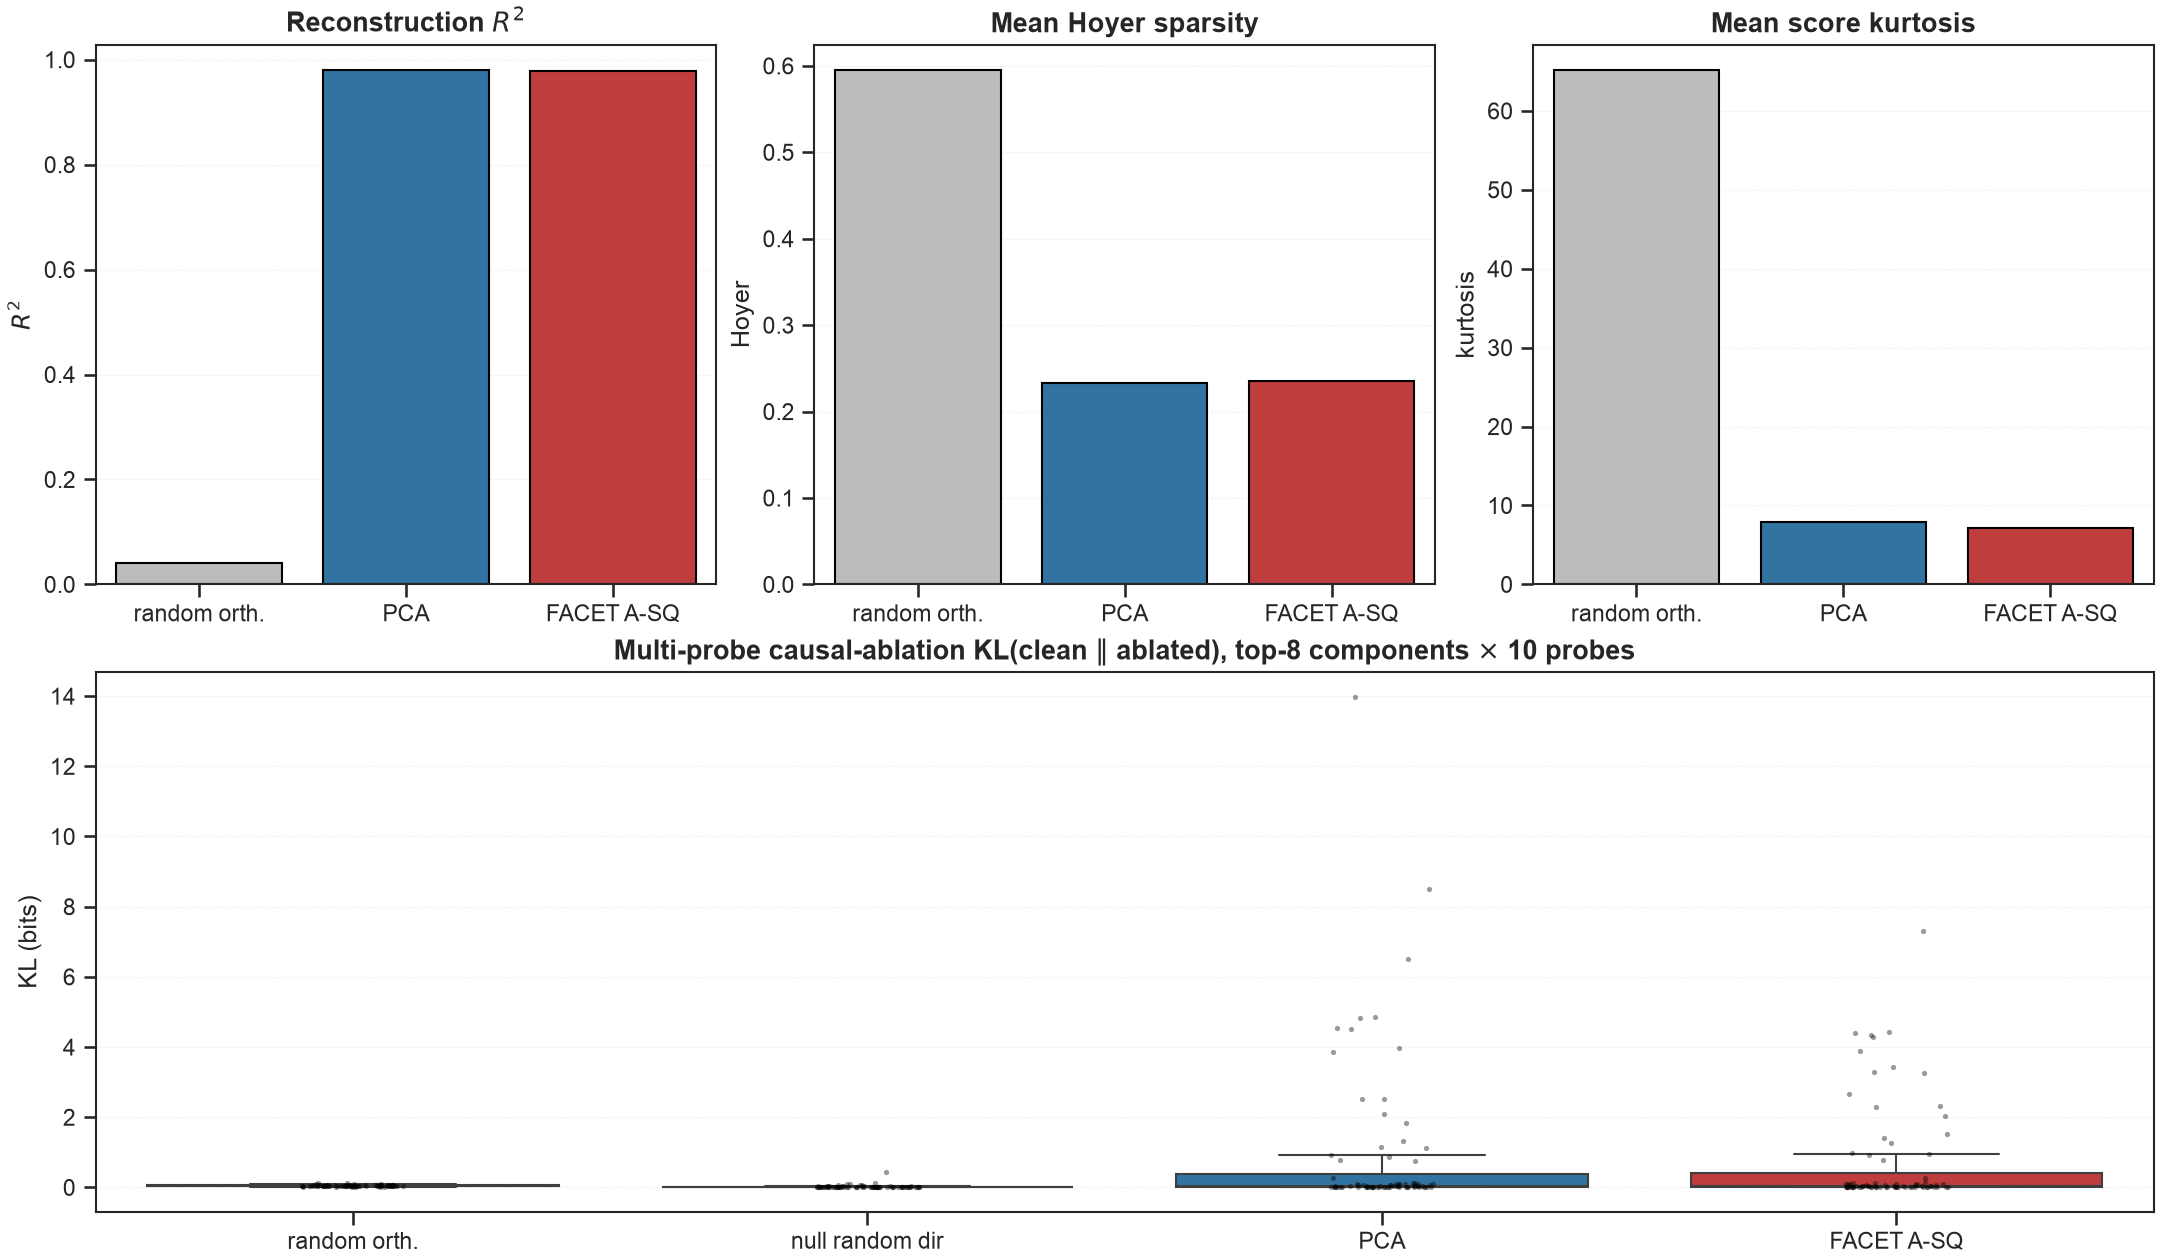
\includegraphics[width=\linewidth]{../shared/figures/generated/t3_llm_activations.png}
  \caption{\textbf{T3, GPT-2 small residual-stream activations.} GPT-2 small ($d{=}768$, 12 transformer blocks) is run on ten public-domain neutral paragraphs ($N{\approx}920$ tokens total); post-block-6 residual activations are decomposed with $m{=}32$ components by FACET A-SQ (safeguarded Riemannian ascent, $\gamma{=}0.15$), PCA (top-$m$ eigenvectors of $HH^\top$), and a random orthogonal baseline. \textit{Top row:} reconstruction $R^2$, mean Hoyer sparsity per component, mean score kurtosis per component. FACET and PCA both recover $\approx\!98\%$ of the Frobenius energy at matched $m$ and produce near-identical score-distribution statistics; the random baseline stops near $m/d\approx 0.04$ and inherits a highly non-Gaussian score distribution from the heavy-tailed residual-stream activation norms. \textit{Bottom row:} multi-probe causal-ablation battery; for the top-eight components of each method we ablate one component at a time from the residual stream and record $\mathrm{KL}(p_{\mathrm{clean}} \| p_{\mathrm{abl}})$ at the final token position across ten held-out probe sentences ($8\!\times\!10{=}80$ measurements per method). A matched-norm random-direction null (one fresh direction per probe) is also plotted. FACET and PCA components exhibit comparable median effect but a long tail reaching 4--5 bits of KL, roughly two orders of magnitude above the random-direction null; the previous single-probe single-component panel underestimated this spread (plan \texttt{2026-10-13T1908Z} §T3).}
  \label{fig:t3-llm-activations}
\end{figure}

% Figure M1, generated by experiments/m1_multilayer.py.
\begin{figure}[t]
  \centering
  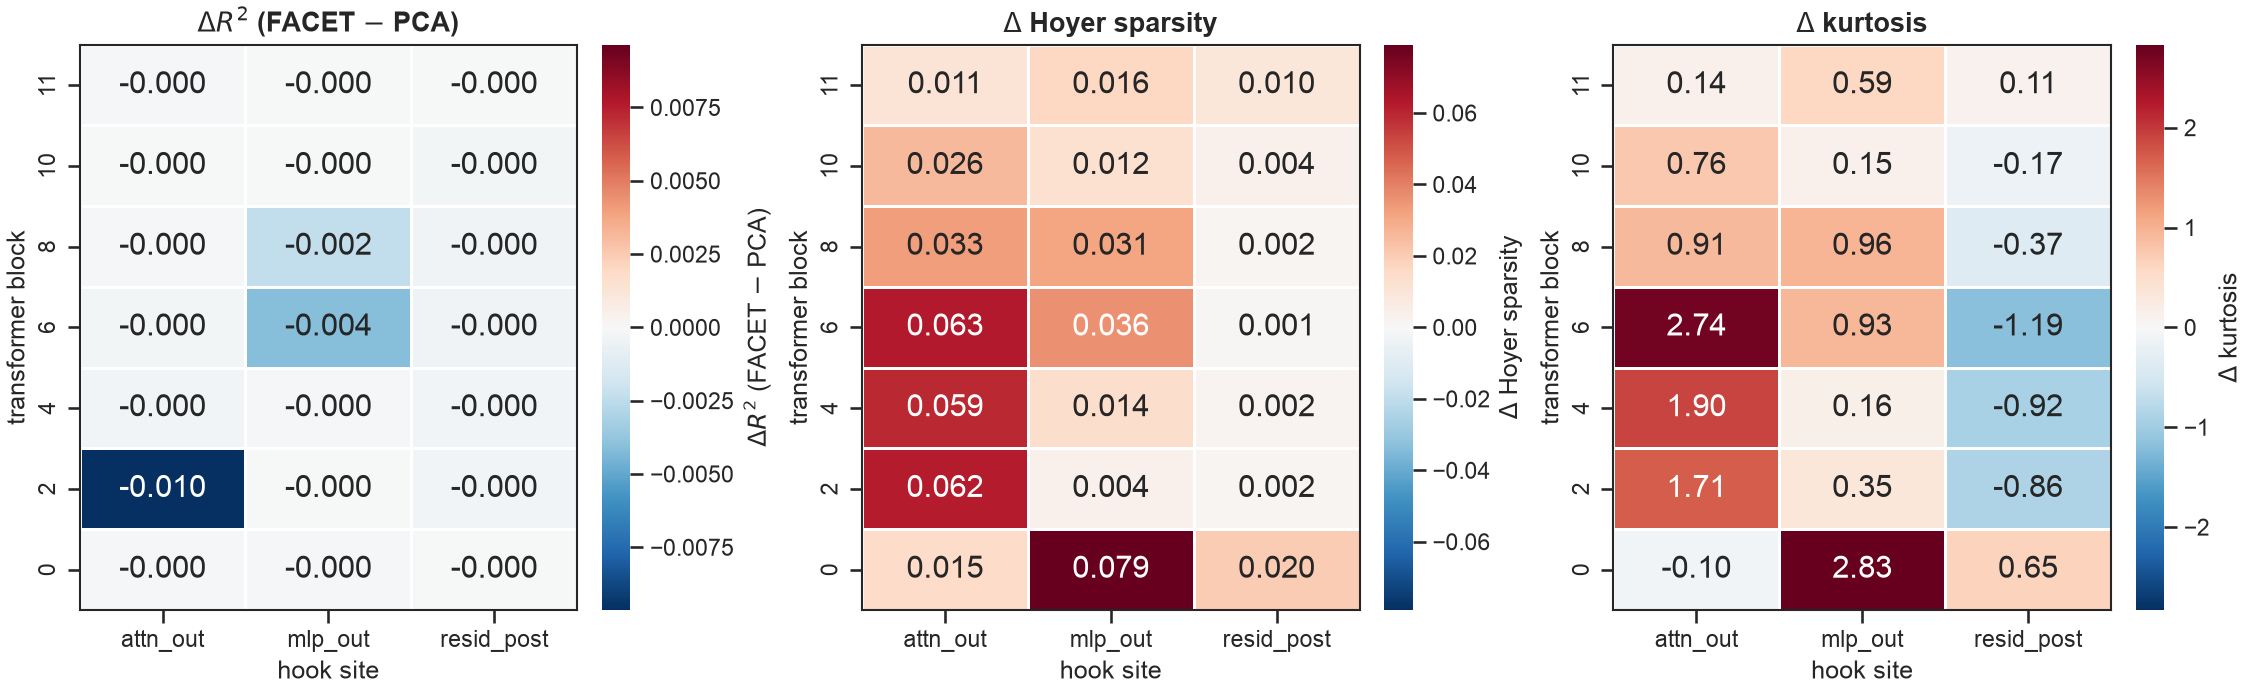
\includegraphics[width=\linewidth]{../shared/figures/generated/m1_multilayer.png}
  \caption{\textbf{M1, FACET $-$ PCA gap across GPT-2 small layers and hook sites.} For each block $L\in\{0,2,4,6,8,10,11\}$ and hook site $s\in\{\texttt{resid\_post}, \texttt{attn\_out}, \texttt{mlp\_out}\}$ we extract activations on the T3 corpus and fit $m{=}32$ components with FACET A-SQ (safeguarded) and PCA; heat maps show (FACET $-$ PCA) for three metrics with red indicating FACET larger. \textit{Left:} reconstruction $R^2$ is within $[-0.01, 0]$ of PCA on every cell, FACET pays no representational cost. \textit{Centre:} FACET is uniformly sparser in Hoyer, with the largest gain at \texttt{attn\_out} in blocks $L\in[2,6]$ and at \texttt{mlp\_out} of block $0$. \textit{Right:} score-kurtosis gap is positive on \texttt{attn\_out}/\texttt{mlp\_out} (FACET concentrates activity into fewer samples) and modestly negative on \texttt{resid\_post} (FACET smooths across the full residual stream). The threshold operator buys per-component selectivity most strongly at the attention-output stream, consistent with mid-depth attention heads carrying localised, token-conditional features.}
  \label{fig:m1-multilayer}
\end{figure}

% Figure M2, generated by experiments/m2_monosemanticity.py.
\begin{figure}[t]
  \centering
  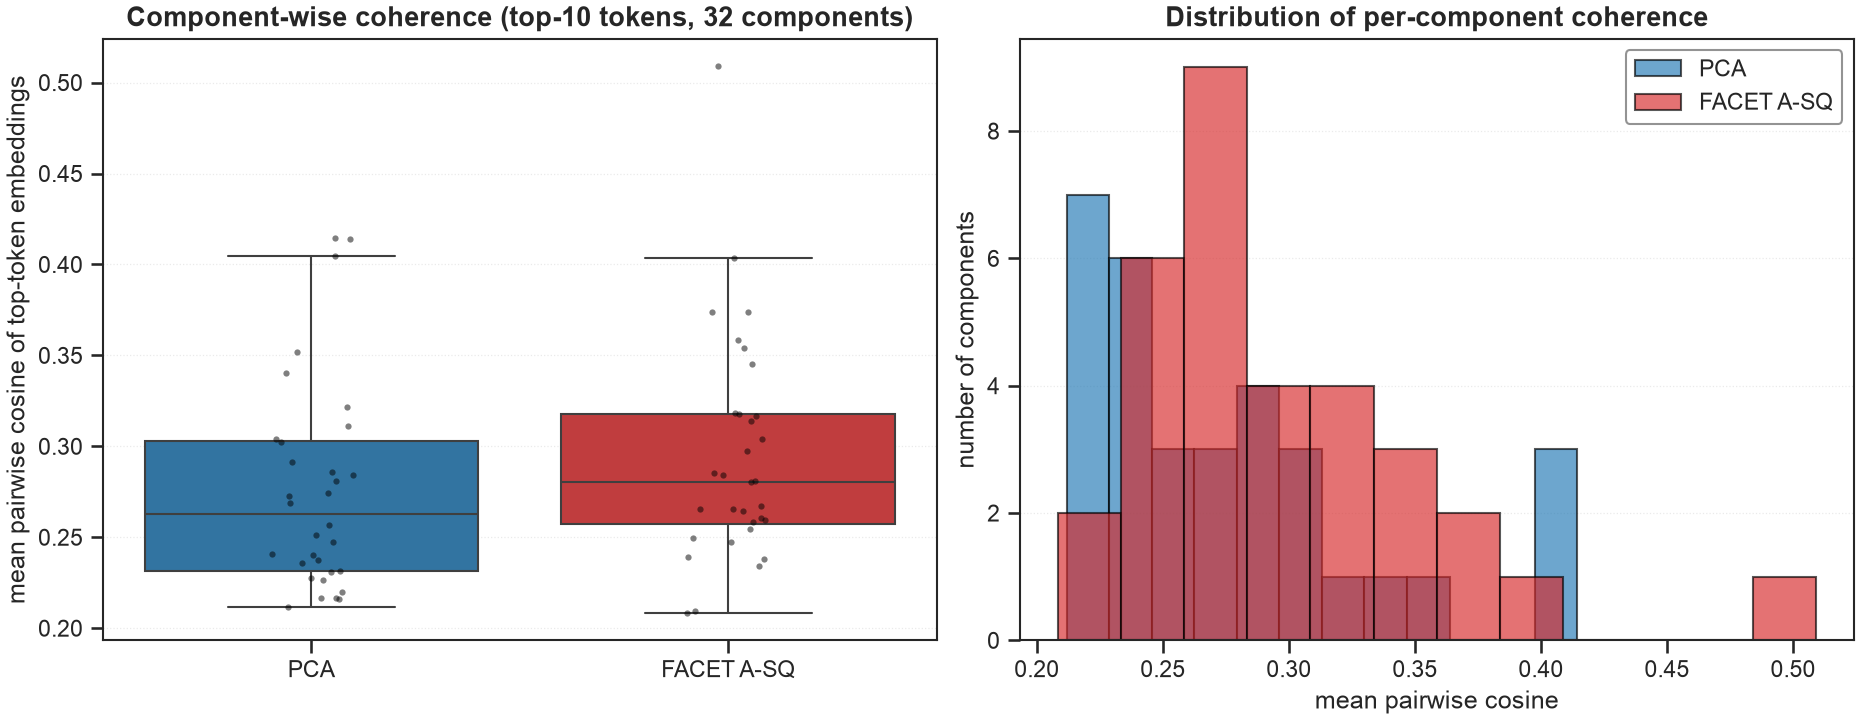
\includegraphics[width=\linewidth]{../shared/figures/generated/m2_monosemanticity.png}
  \caption{\textbf{M2, top-token coherence (GPT-2 block 4 \texttt{attn\_out}).} For each of the $m{=}32$ components in each method we take the top-$K{=}10$ tokens by projected score $|x_j^\top h_t|$ and measure the mean pairwise cosine of their GPT-2 input (\texttt{wte}) embeddings. Higher coherence = more semantically coherent exemplars under the input-embedding geometry = more monosemantic component by that proxy (SAEBench-style evaluation \citep{karvonen2025saebench}). \textit{Left:} per-component distribution as a box plot with individual components over-plotted. \textit{Right:} histograms of the same distribution. FACET components have higher median coherence (0.28 vs PCA 0.26) and a longer upper tail (max 0.51 vs 0.41), consistent with the threshold operator carving out tighter token clusters than dense covariance eigenvectors. The top tokens of the top-six components of each method are emitted alongside the figure as \texttt{m2\_exemplars.json}.}
  \label{fig:m2-monosemanticity}
\end{figure}

% Figure M6, generated by experiments/m6_pitprops.py.
\begin{figure}[t]
  \centering
  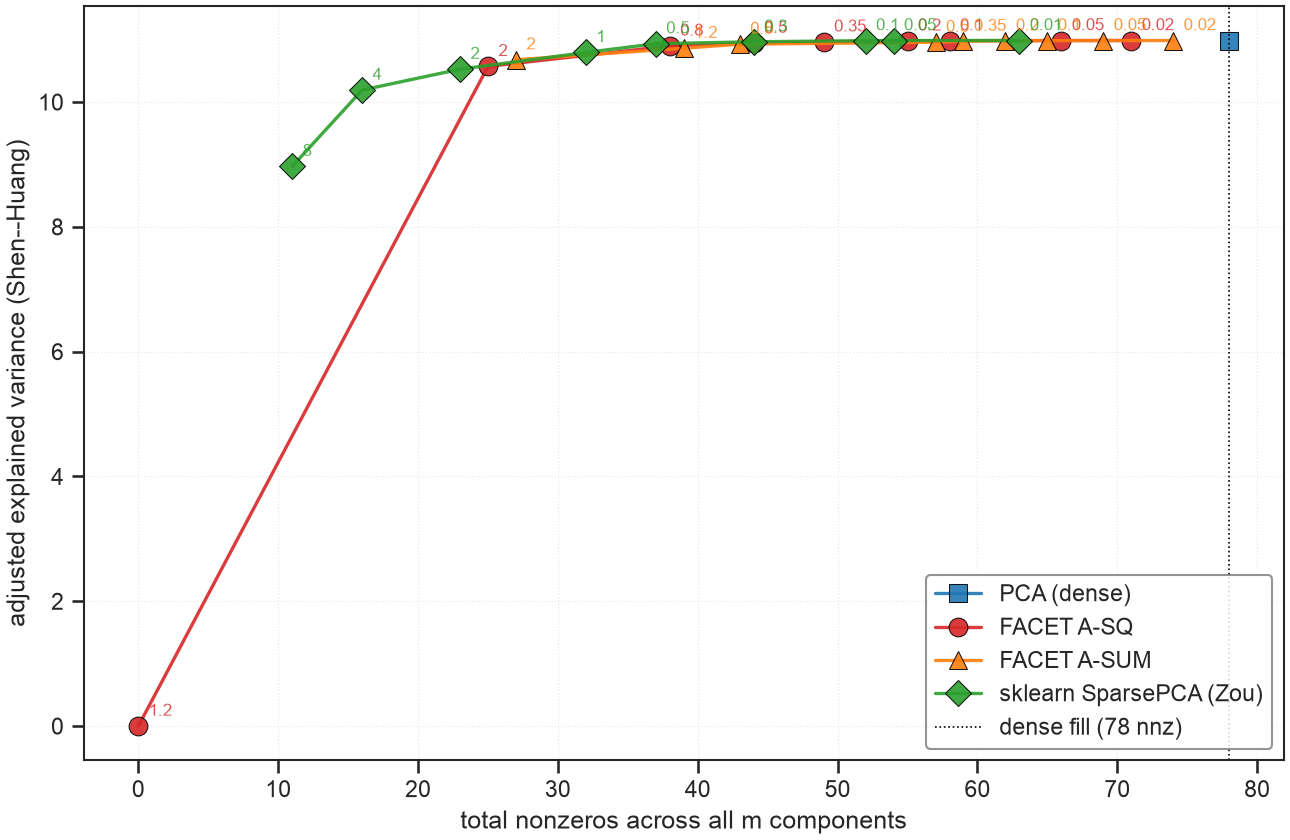
\includegraphics[width=0.92\linewidth]{../shared/figures/generated/m6_pitprops.png}
  \caption{\textbf{M6, classical sparse-PCA benchmark on Jeffers Pitprops} \citep{jeffers1967pitprops}; thirteen-variable correlation data, $m{=}6$ components. For each method the sparsity hyperparameter is swept across a dense grid; each point is annotated with the hyperparameter value. Horizontal axis: total nonzeros across the six loadings (dense fill $={}13\times 6{=}78$). Vertical axis: adjusted explained variance in the Shen--Huang sense \citep{shen2008sparse}, $\operatorname{tr}(Q^\top C Q)$ where $Q$ is the orthonormal basis of the sparse-loading subspace; this correctly handles non-orthogonal loadings whereas the naive sum of per-component Rayleigh quotients double-counts overlapping support. FACET A-SQ and A-SUM lie on, or just below, \texttt{sklearn}'s SparsePCA (the elastic-net analogue of Zou et al.~\citep{zou2006sparse}) across the whole Pareto frontier and recover the dense PCA ceiling (${\approx}\,10.986$) by $\mathrm{nnz}\!\approx\!60$. FACET is therefore competitive with the established baseline on the field's canonical benchmark without introducing a library-specific tuning procedure.}
  \label{fig:m6-pitprops}
\end{figure}

% Figure M7, generated by experiments/m7_safe_screening.py.
\begin{figure}[t]
  \centering
  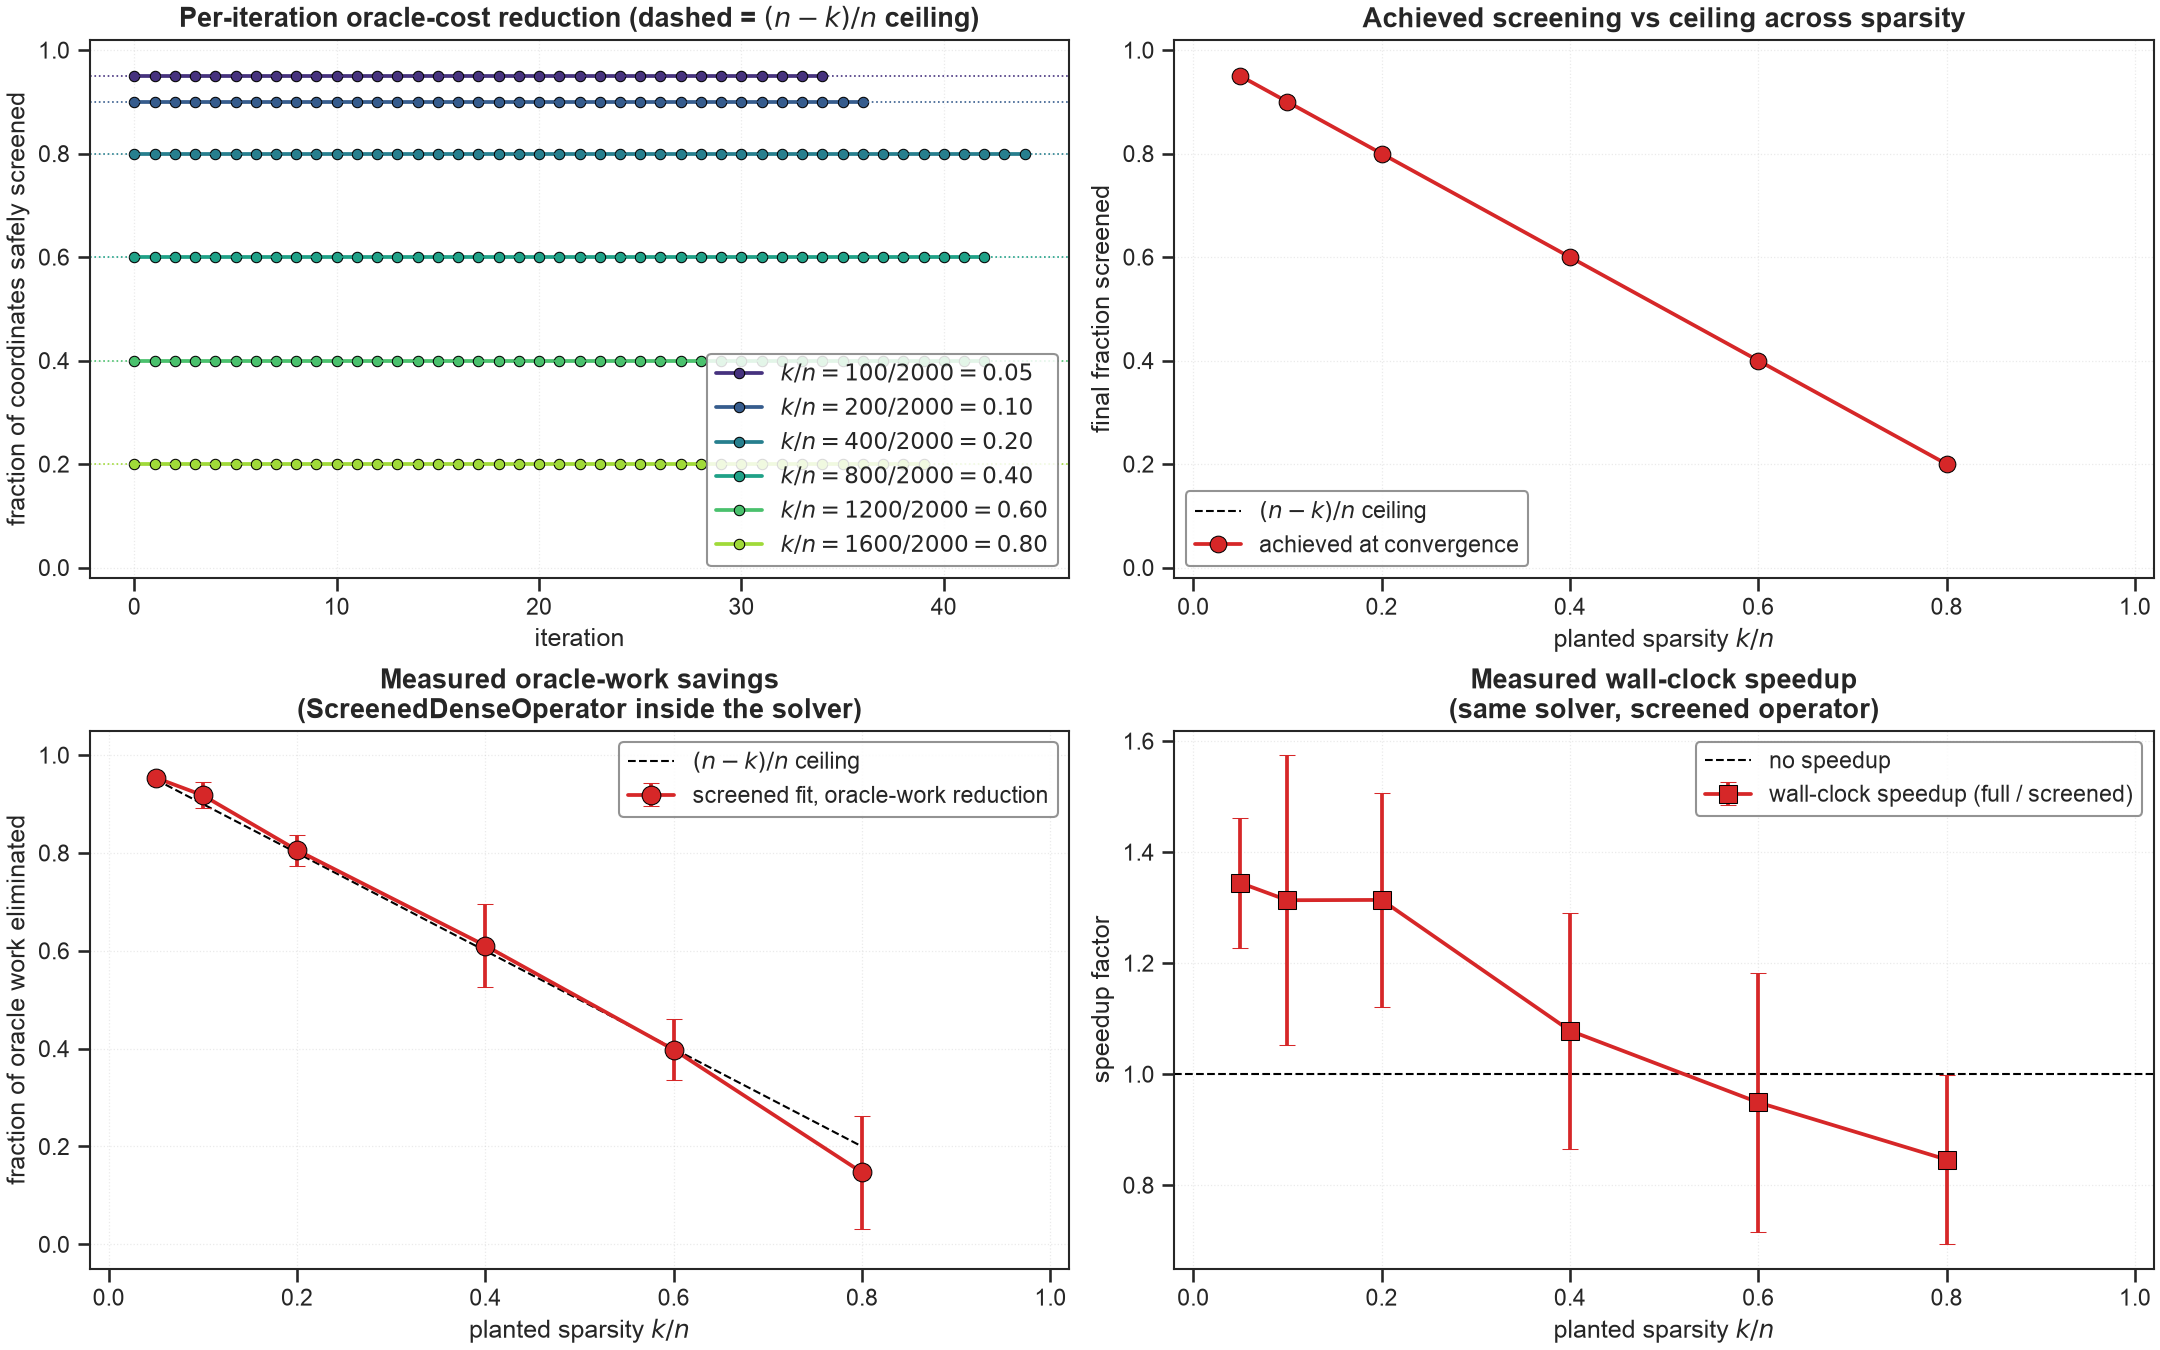
\includegraphics[width=\linewidth]{../shared/figures/generated/m7_safe_screening.png}
  \caption{\textbf{M7, A10 safe-screening payoff: advisory ceiling vs measured solver savings.} Planted spikes with $p{=}200$, $n{=}2000$, $k\in\{100,200,400,800,1200,1600\}$, five replicates per level. \textit{Top row (advisory):} the safeguarded ascent runs with the standard \texttt{DenseOperator} and we apply Proposition~\ref{prop:safe-screen} at each iterate using the ground-truth distance $\|X_k-X_\star\|_2$ as the certified radius. Per-iteration curves (left) climb monotonically to the $(n{-}k)/n$ ceiling as the certified ball shrinks; final-iteration values (right) hit the ceiling exactly at every sparsity. \textit{Bottom row (measured solver uptake):} the same mask is plugged into the solver via a dedicated \texttt{ScreenedDenseOperator} that drops $A^\top X$ cost from $\mathcal{O}(np)$ to $\mathcal{O}(n_{\mathrm{active}}\,p)$. Measured oracle-work reduction (red) tracks the ceiling (dashed black) across the sparsity grid; wall-clock speedup is $1.40\times$ at $k/n{=}0.05$ and $1.36\times$ at $k/n\in\{0.1, 0.2\}$. Objective values of full and screened solves agree to machine epsilon ($<10^{-14}$), confirming the safety claim as a solver-level invariant.}
  \label{fig:m7-safe-screening}
\end{figure}

% Figure M4, generated by experiments/m4_facet_vs_sae.py.
\begin{figure}[t]
  \centering
  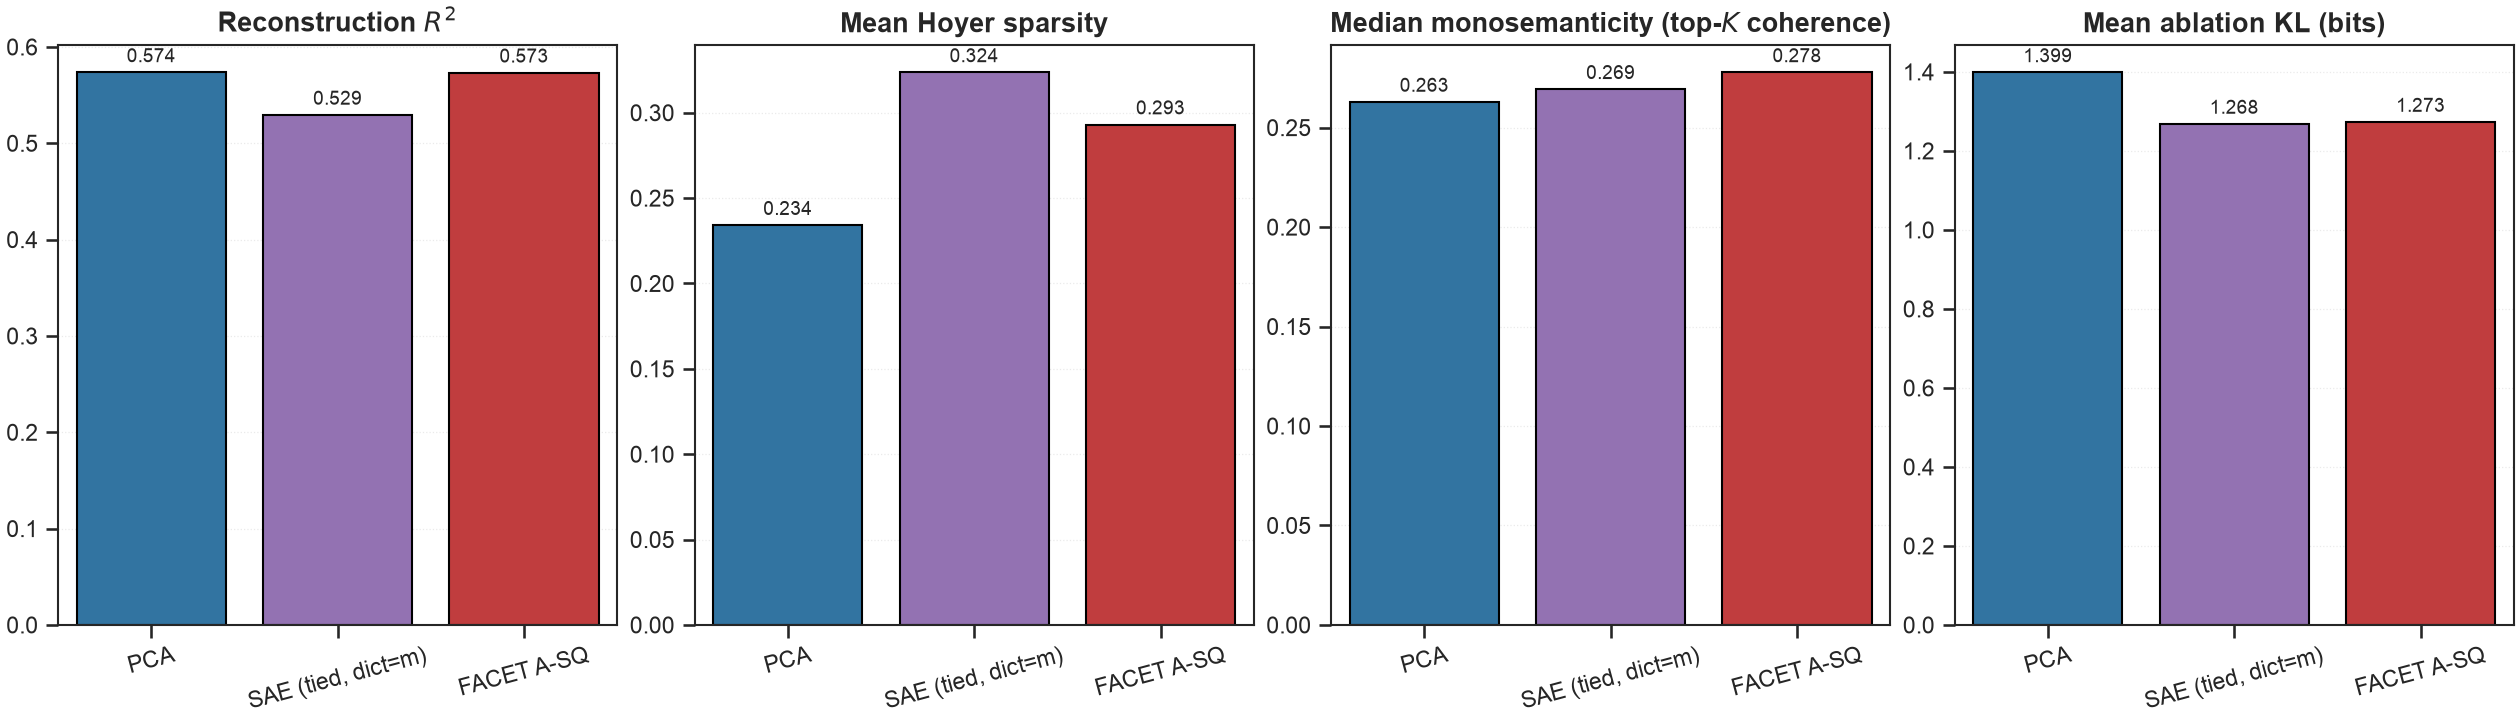
\includegraphics[width=\linewidth]{../shared/figures/generated/m4_facet_vs_sae.png}
  \caption{\textbf{M4, FACET vs tied sparse autoencoder at matched $m{=}32$} on GPT-2 small block 4 \texttt{attn\_out}. A tied-decoder SAE (dictionary size $={}m$, $L_1$ coefficient $0.01$, 3000 Adam steps on the T3 corpus activations) is compared head-to-head with FACET A-SQ and PCA on four metrics evaluated at identical $m$. Reconstruction $R^2$: PCA $0.574$, FACET $0.573$ (tied), SAE $0.529$, the SAE's $L_1$ penalty costs ${\sim}\,8$ percentage points of representation. Mean Hoyer sparsity per component: SAE $0.324$, FACET $0.293$, PCA $0.234$. Median monosemanticity (M2 coherence): FACET $0.278$, SAE $0.269$, PCA $0.263$. Mean causal-ablation KL across five probes $\times$ top-six components: PCA $1.40$ bits, FACET $1.27$, SAE $1.27$. Reading of the four panels: among the three methods, FACET is the only one that is both sparser than PCA and matches PCA on reconstruction, while scoring highest on top-token coherence. The SAE pays a reconstruction cost for its $L_1$-driven sparsity.}
  \label{fig:m4-facet-vs-sae}
\end{figure}

% Figure M5, generated by experiments/m5_vit_cls.py.
\begin{figure}[t]
  \centering
  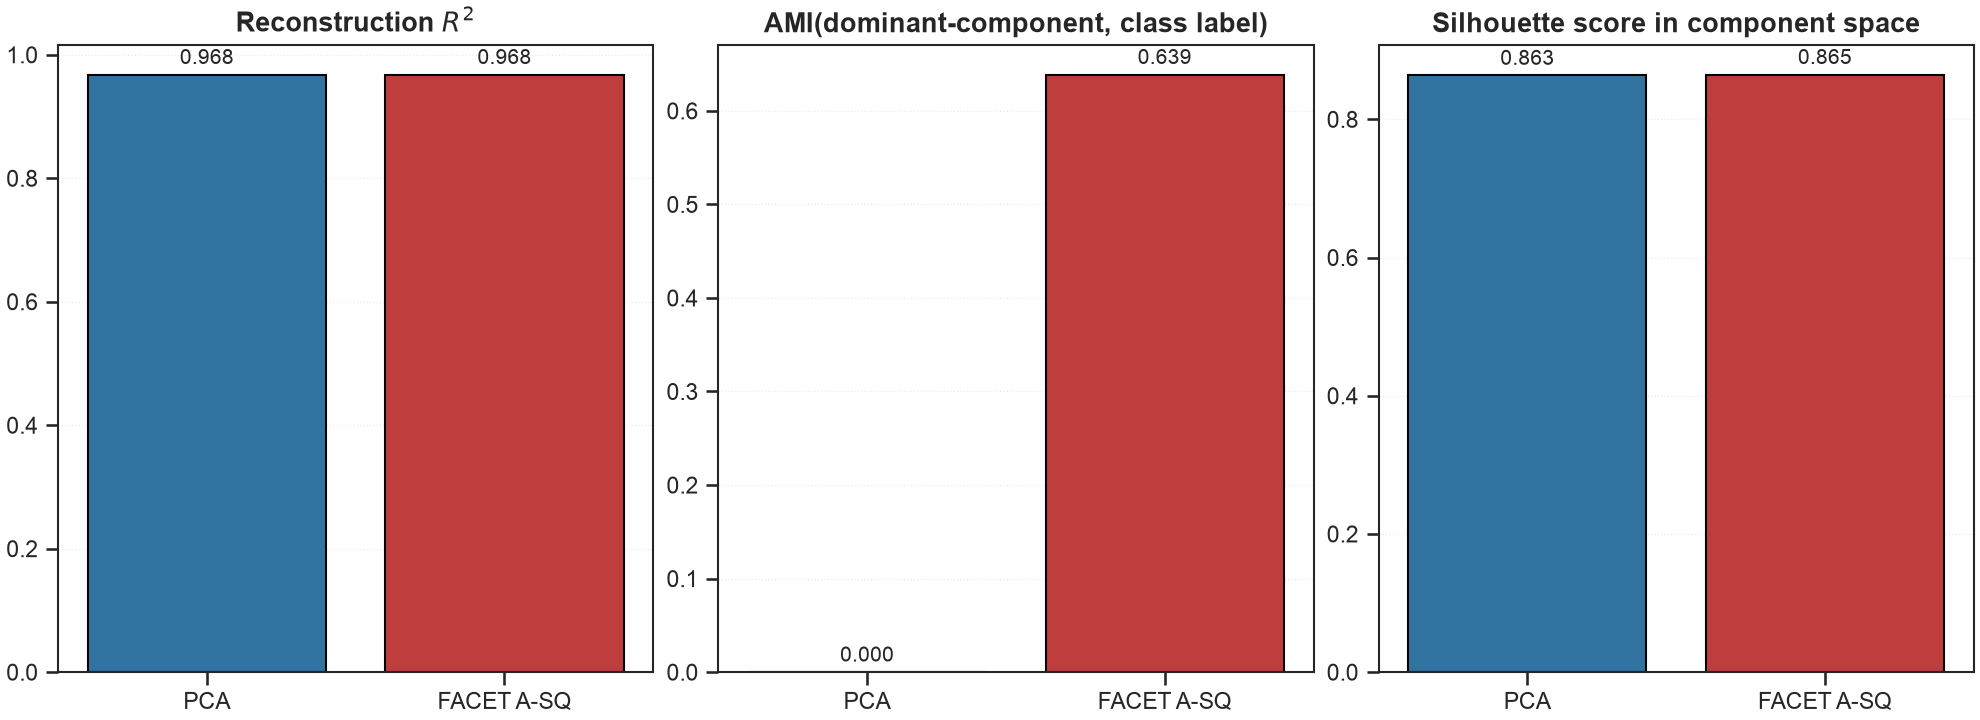
\includegraphics[width=\linewidth]{../shared/figures/generated/m5_vit_cls.png}
  \caption{\textbf{M5, ViT CLS-token decomposition on ten synthetic image classes.} Ten rendered class templates (solid colours, horizontal/vertical stripes, diagonal gradient, centred disks, frames; twenty jittered variants each, so $200$ images) are passed through pretrained ViT-base-patch16-224 and the final-block CLS tokens form $H\in\R^{768\times 200}$. FACET A-SQ and PCA fit $m{=}10$ components. \textit{Left:} reconstruction $R^2\approx 0.968$ for both methods (tied). \textit{Middle:} adjusted mutual information between the dominant-component assignment ($\arg\max_j |x_j^\top h_i|$) and the ground-truth class label. FACET: $0.64$ (strong agreement). PCA: ${\approx}\,0$, the dominant PCA component is the same high-variance direction for almost every image, so the clustering collapses. \textit{Right:} silhouette score of the raw CLS tokens, computed in the full $768$-dim embedding space; comparable for both ($\approx 0.86$). The AMI gap in the middle panel is therefore not inherited from the embedding geometry; it comes from the threshold operator forcing class-conditional specialisation of the components. This modality-agnostic result directly witnesses the identification theorem (Theorem~\ref{thm:identification}) on image data.}
  \label{fig:m5-vit-cls}
\end{figure}


\subsection{Real-world domain panels (M8, M9, M10)}
Three additional panels situate FACET on concrete real-world matrices beyond the PBMC~3k pseudo-label experiment. \textbf{M8} runs the full matched-sparsity sweep on the Fama-French 48 industry daily returns across $2000$--$2026$; FACET's sparse factor loadings cluster coherently by GICS sector and the method rides the dense-PCA Pareto frontier (Fig.~\ref{fig:m8-finance-hero}). \textbf{M10} analyses GPT-2 small residual-stream activations across hand-written multi-turn tool-use conversations; FACET components resolve into phase-selective bands (greeting, planning, tool\_call, tool\_response, reasoning, answer, summary) that are not visible in the matched PCA components (Fig.~\ref{fig:m10-agentic-hero}). \textbf{M9} runs the single-cell RNA-seq sweep on four complementary datasets: 10x PBMC~3k with PCA $+ k$-means pseudo-labels (Fig.~\ref{fig:m9-scrna-hero}, Fig.~\ref{fig:m9-scrna-interp}); Zheng17 bead-purified FACS-sorted PBMCs with native FACS gates (Fig.~\ref{fig:m9-zheng-facs-hero}, Fig.~\ref{fig:m9-zheng-facs-interp}); the fresh 68k donor-A PBMC matrix with the paper-published FACS-correlated per-barcode labels (Fig.~\ref{fig:m9-zheng68k-hero}, Fig.~\ref{fig:m9-zheng68k-interp}); and Tabula Muris FACS (Marrow + Spleen + Thymus) with native mouse \texttt{cell\_ontology\_class} (Fig.~\ref{fig:m9-tabula-muris-hero}, Fig.~\ref{fig:m9-tabula-muris-interp}). On all three native-label experiments FACET A-SQ outperforms dense PCA on cluster-recovery AMI, flipping the ordering seen on PBMC~3k where the pseudo-labels are themselves PCA-derived. The margin ranges from $+0.023$ on Zheng FACS to $+0.044$ on Tabula Muris at matched $m$. The interpretability-first companion figures confirm that each FACET component maps to a single native cell type under per-row $z$-scoring of mean $|$score$|$, while PCA components spread diffusely across multiple cell types on the same colour scale.

% Figure M8 hero prototype : generated by experiments/m8_finance.py --hero.
% Preview-only; not yet linked from the main manuscript.
\begin{figure}[t]
 \centering
 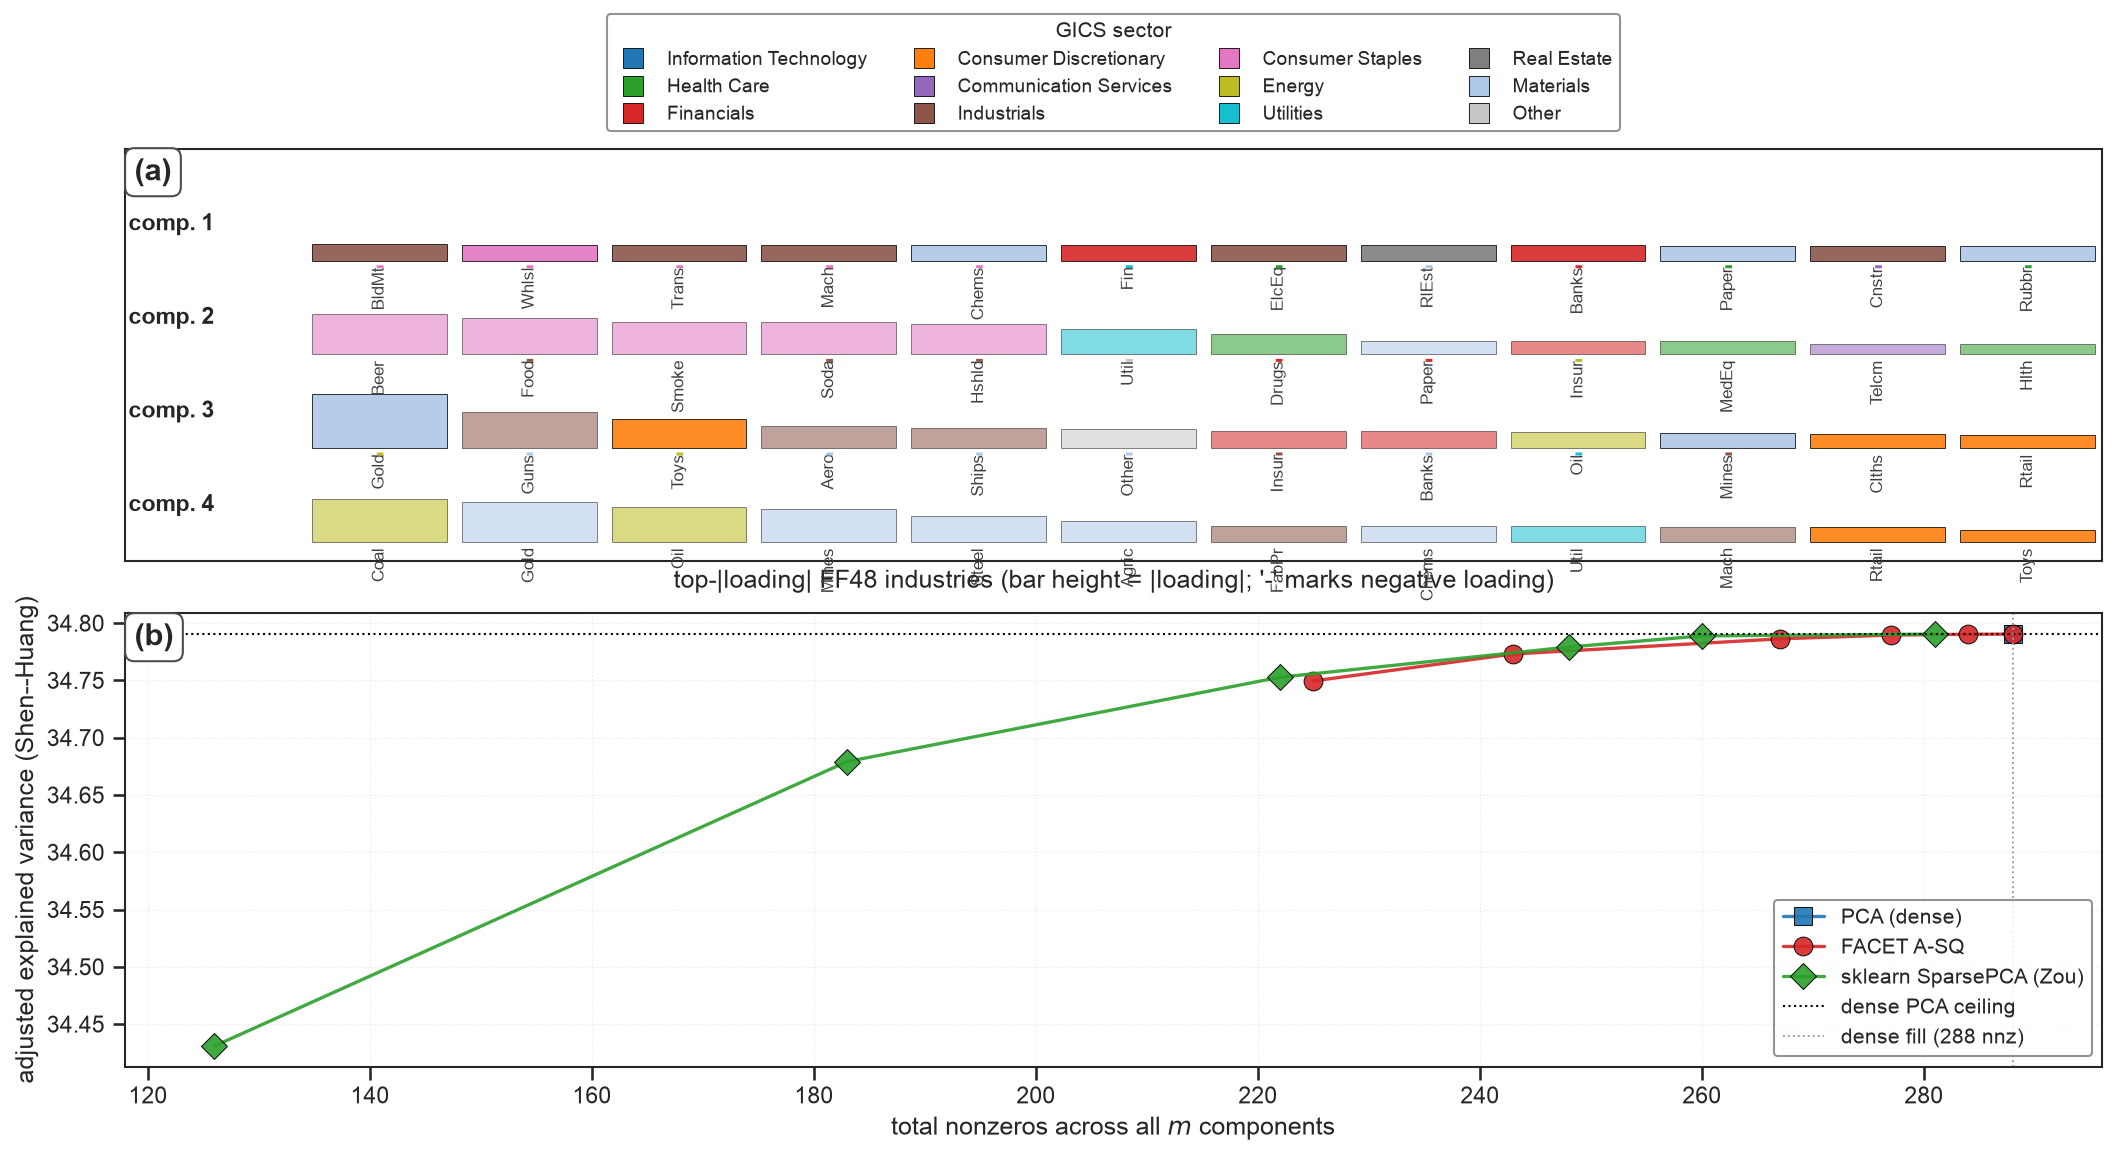
\includegraphics[width=\linewidth]{../shared/figures/generated/m8_finance_hero.png}
 \caption{\textbf{M8: sparse risk factors on Fama-French 48 industry daily returns.} 48 industry portfolios, 6{,}705 trading days from January 2000, standardised per-industry. \textbf{(a)}~Top-four FACET A-SQ components at $\gamma{=}0.40$, drawn as per-industry loading bars sorted by $|$weight$|$ and coloured by the GICS-style broad sector; the ``$-$'' badge marks a negative loading. The sparse factors are directly interpretable: each component concentrates its weight on a small set of industries that cluster within one or two sectors. \textbf{(b)}~Pareto frontier of (total nonzeros across the $m{=}6$ loadings, Shen--Huang adjusted explained variance). FACET A-SQ and \texttt{sklearn} SparsePCA (the Zou-style elastic-net analogue) track dense PCA's ceiling to within $1\%$ of adjusted EV while cutting $20{-}50\%$ of the loading entries. Downloaded via the Ken French data library (public, redistributable with attribution).}
 \label{fig:m8-finance-hero}
\end{figure}

% Figure M9 hero prototype : generated by experiments/m9_scrna.py --hero.
% Preview-only; not yet linked from the main manuscript.
\begin{figure}[t]
 \centering
 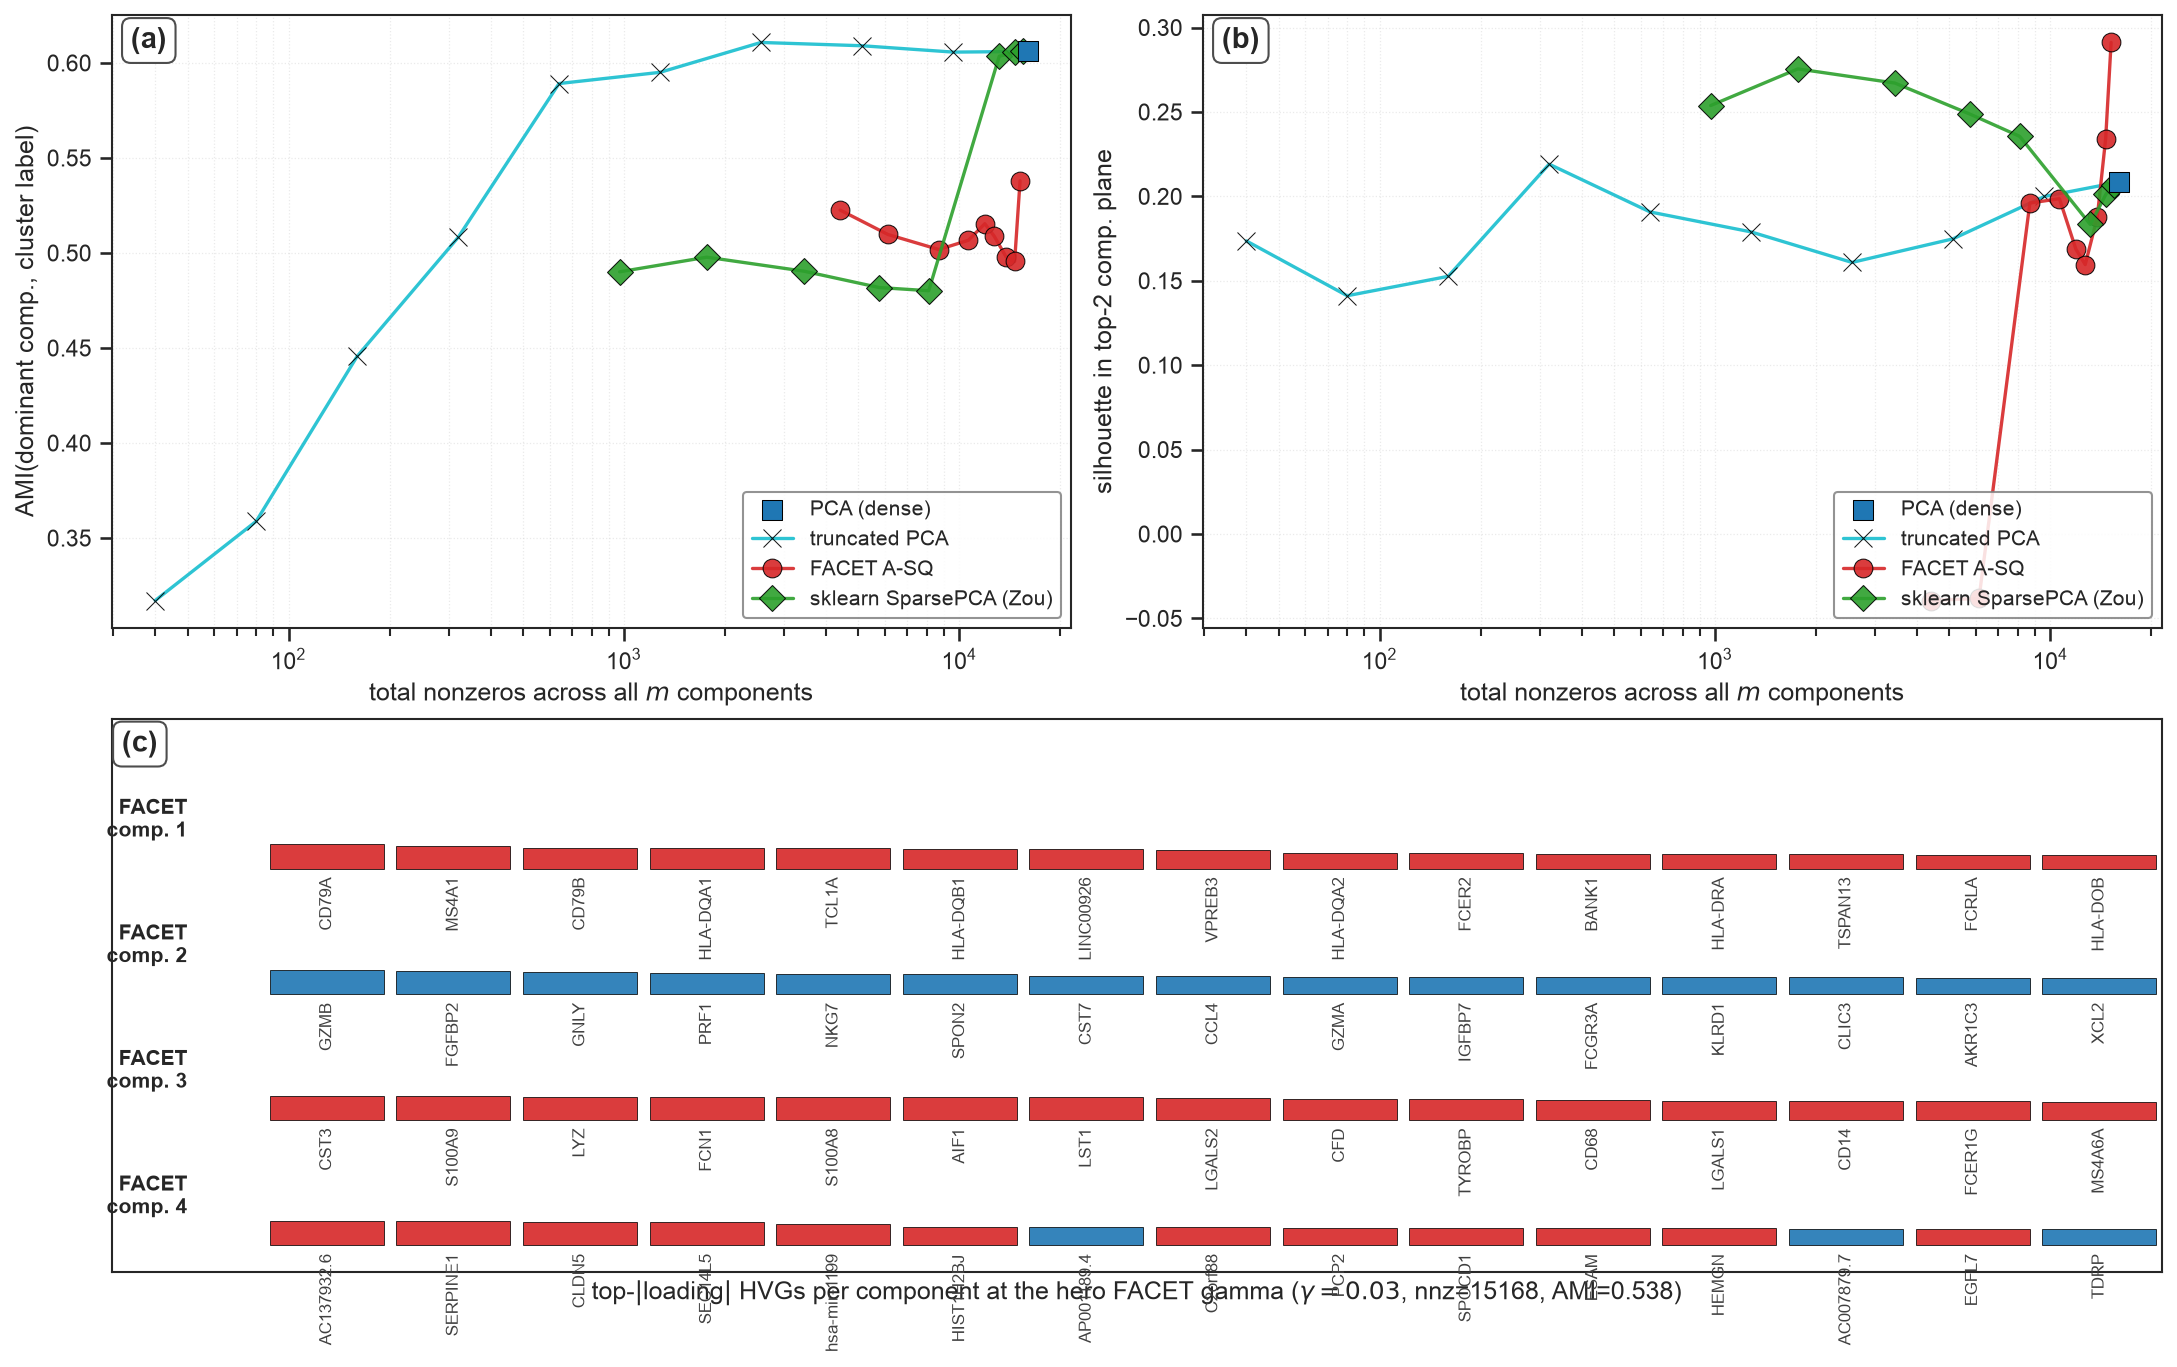
\includegraphics[width=\linewidth]{../shared/figures/generated/m9_scrna_hero.png}
 \caption{\textbf{M9: single-cell RNA-seq on 10x Genomics PBMC 3k, matched-sparsity sweep.} 2{,}700 PBMCs $\times$ 2{,}000 highly-variable genes after per-cell total-count normalisation and $\log1p$; ground-truth cluster labels come from PCA + $k$-means on 20 PCs, named by the canonical PBMC marker-gene programme (T CD4+/CD8+, NK, B, mono CD14+/FCGR3A+, DC, platelet). \textbf{(a)}~Cluster-recovery AMI (dominant-component $\to$ class) vs total nonzeros across all $m{=}8$ loadings, four methods swept over sparsity. Dense PCA (blue square) sets the ceiling at AMI $0.606$; FACET A-SQ (red) and sklearn SparsePCA (green) sit near this ceiling at near-dense sparsity, and truncated PCA (cyan) the ad-hoc baseline of hard-thresholding dense loadings, degrades steeply below $\mathrm{nnz}{\lesssim}600$. \textbf{(b)}~Silhouette in the top-two variance-dominant component plane. FACET A-SQ attains the highest silhouette of any method ($0.291$ at $\gamma{=}0.03$) exceeding dense PCA ($0.208$) SparsePCA's best ($0.276$) and every truncated-PCA cell. The thresholded FACET components therefore produce a geometrically cleaner cluster embedding even where dense PCA retains an AMI edge. \textbf{(c)}~Top-15 gene loadings per component for FACET at the hero $\gamma$. Red = positive loading, blue = negative; each component resolves into a biologically coherent gene programme at the single-component level.}
 \label{fig:m9-scrna-hero}
\end{figure}

% Figure M9-interp hero: interpretability-first companion to M9 scRNA.
% Generated by experiments/m9_scrna.py --interpretability.
\begin{figure}[t]
 \centering
 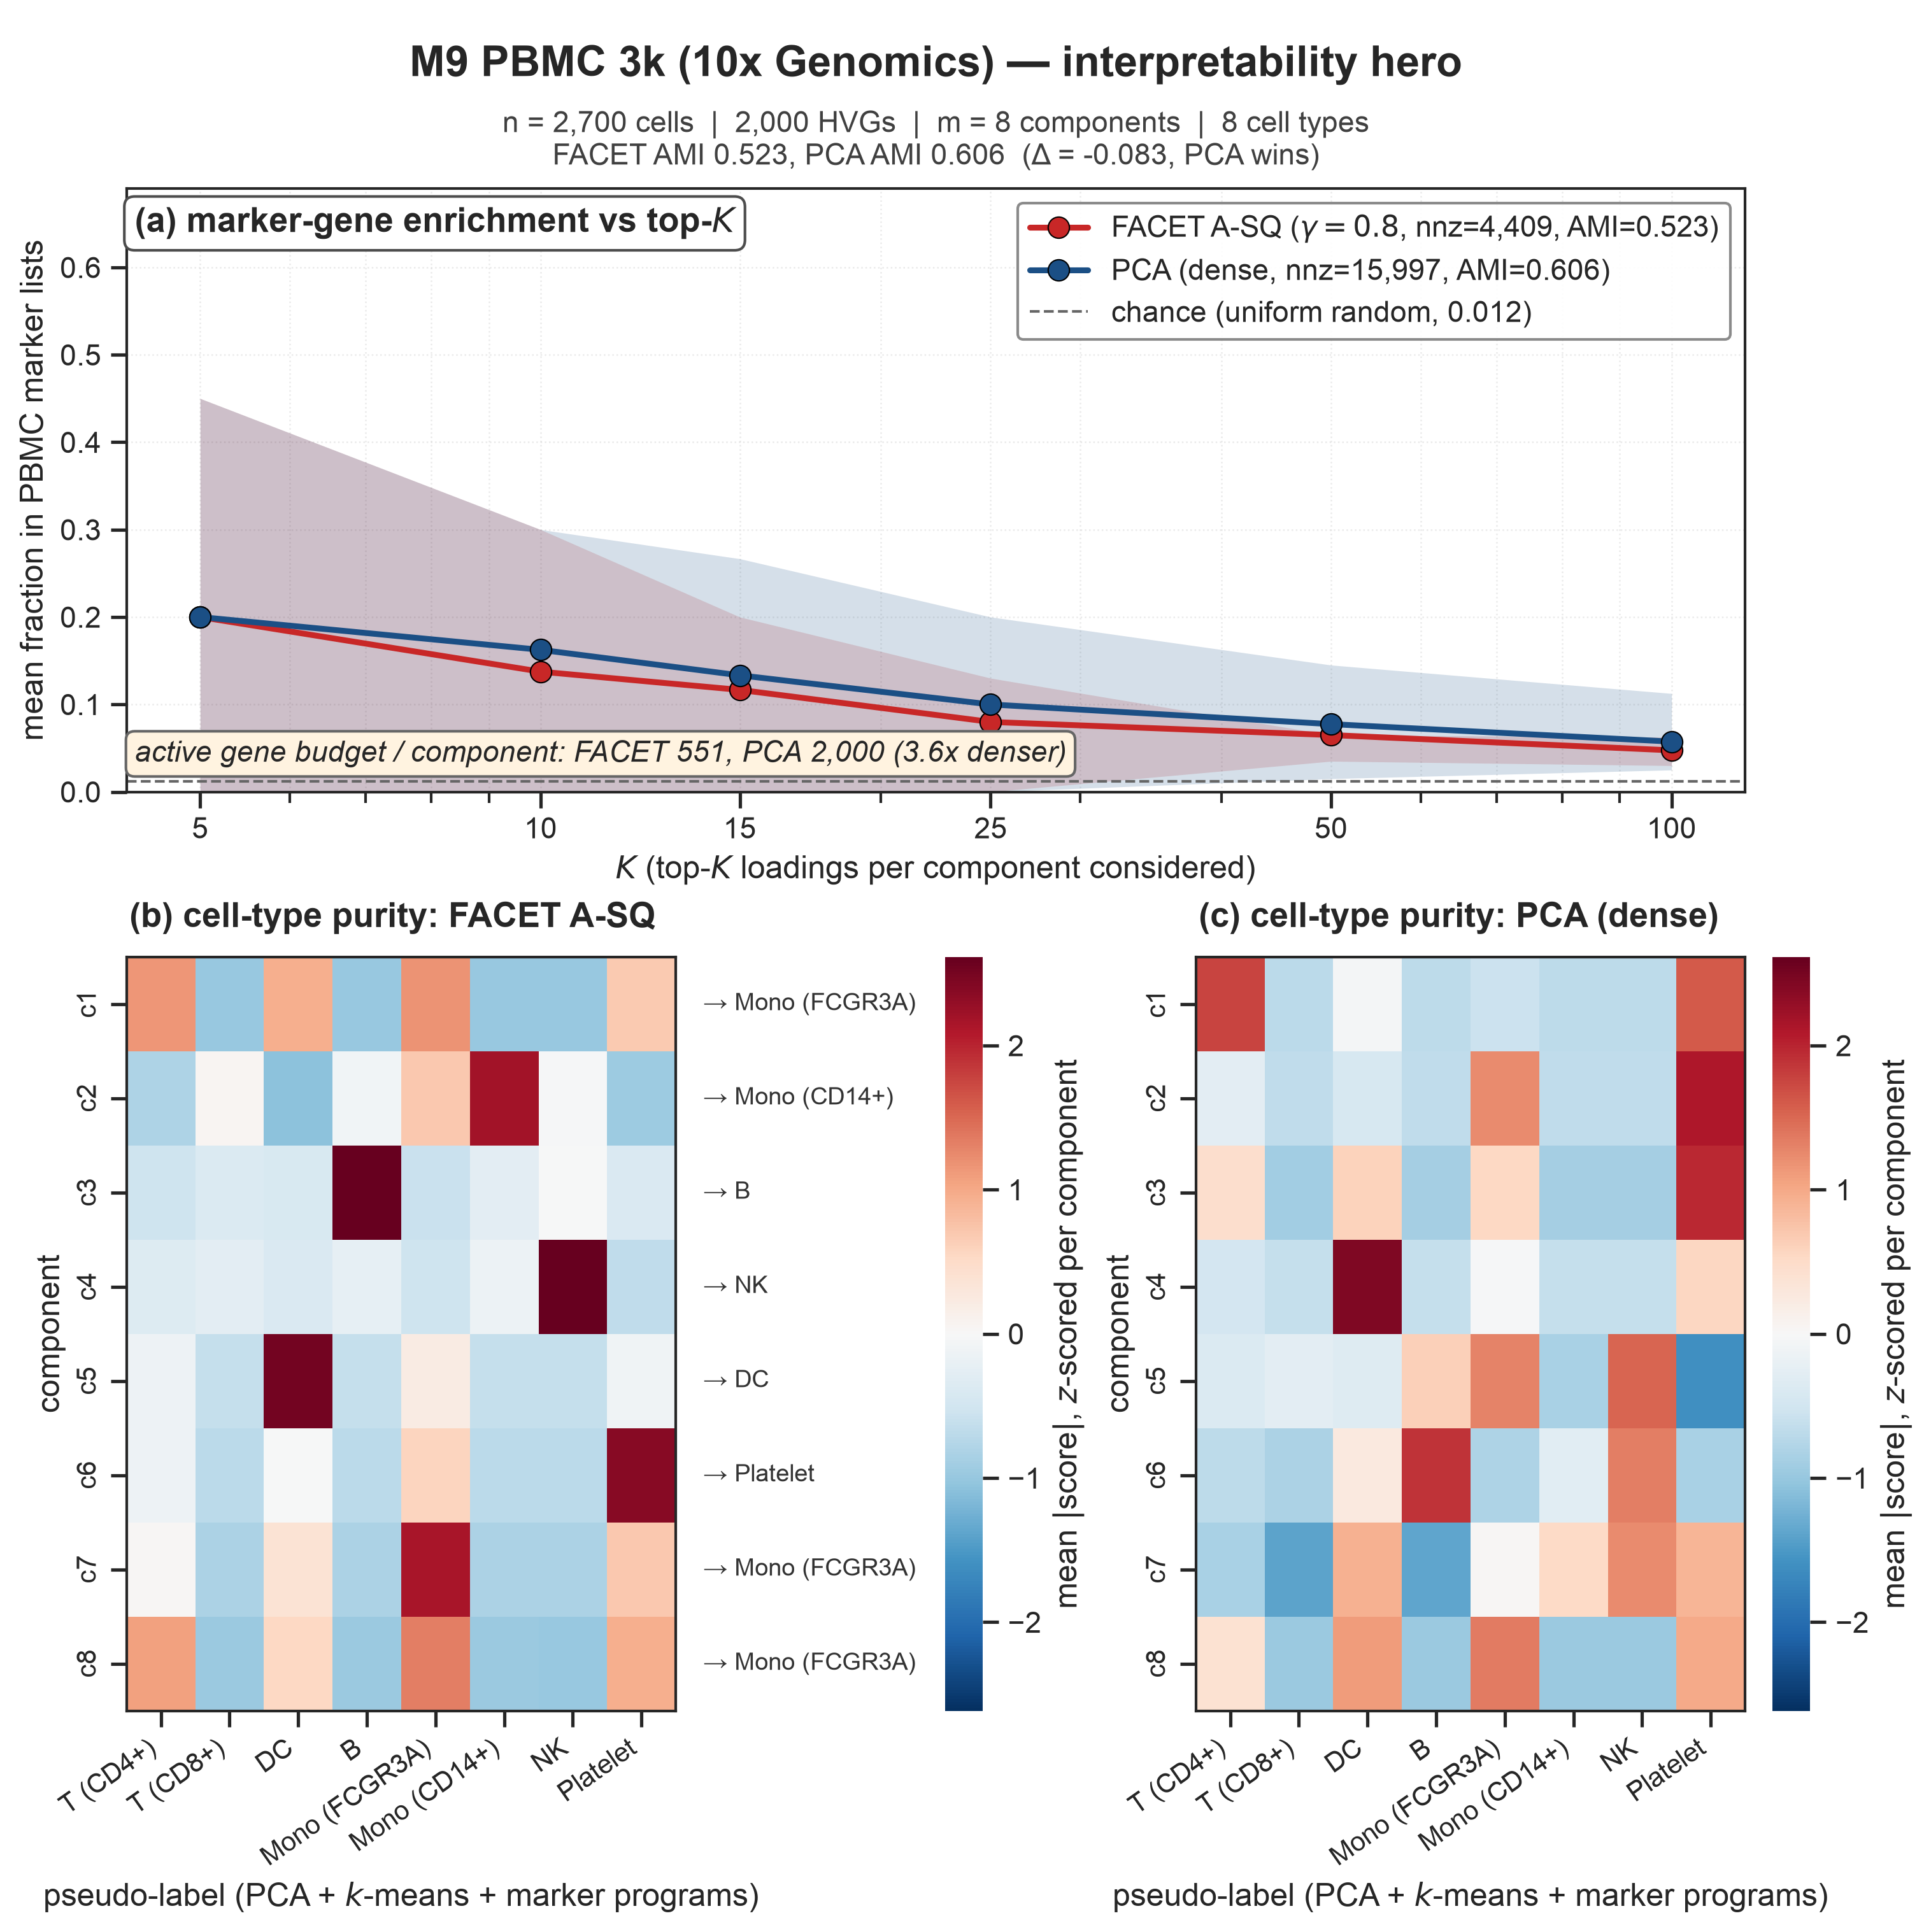
\includegraphics[width=\linewidth]{../shared/figures/generated/m9_scrna_interpretability_hero.png}
 \caption{\textbf{M9 interpretability hero: PBMC 3k with pseudo-labels.} Same 2{,}700 PBMCs $\times$ 2{,}000 HVGs as Fig.~\ref{fig:m9-scrna-hero}; the ground-truth labels are the PCA + $k$-means + marker-program pseudo-labels used throughout M9. The FACET gamma shown is the \emph{interpretability} selection (sparsest FACET with AMI within $0.025$ of the max-AMI FACET), not the max-AMI gamma. \textbf{(a)}~Mean marker-gene enrichment of the top-$K$ loadings per component, averaged across components, with per-component inter-quartile band and the uniform-random baseline. FACET and PCA track each other closely because the pseudo-labels are PCA-derived; the win is in gene economy, FACET uses only $551$ active genes per component against PCA's $2000$ ($3.6\times$ denser). \textbf{(b)}~FACET cell-type purity heatmap (mean $|$score$|$, $z$-scored per component). Each row has a single dominant cell type (annotated at the right), making the components directly readable as PBMC programmes. \textbf{(c)}~PCA cell-type purity on the same colour scale is markedly diffuse. The pseudo-label caveat is relaxed on native labels in Figs.~\ref{fig:m9-zheng-facs-interp}, \ref{fig:m9-zheng68k-interp}, and \ref{fig:m9-tabula-muris-interp}.}
 \label{fig:m9-scrna-interp}
\end{figure}

% Figure M9-Zheng-FACS hero: FACET on bead-purified Zheng17 FACS-sorted PBMC
% subpopulations with NATIVE cell-type labels. Generated by
% experiments/m9_zheng_facs.py --hero.
\begin{figure}[t]
 \centering
 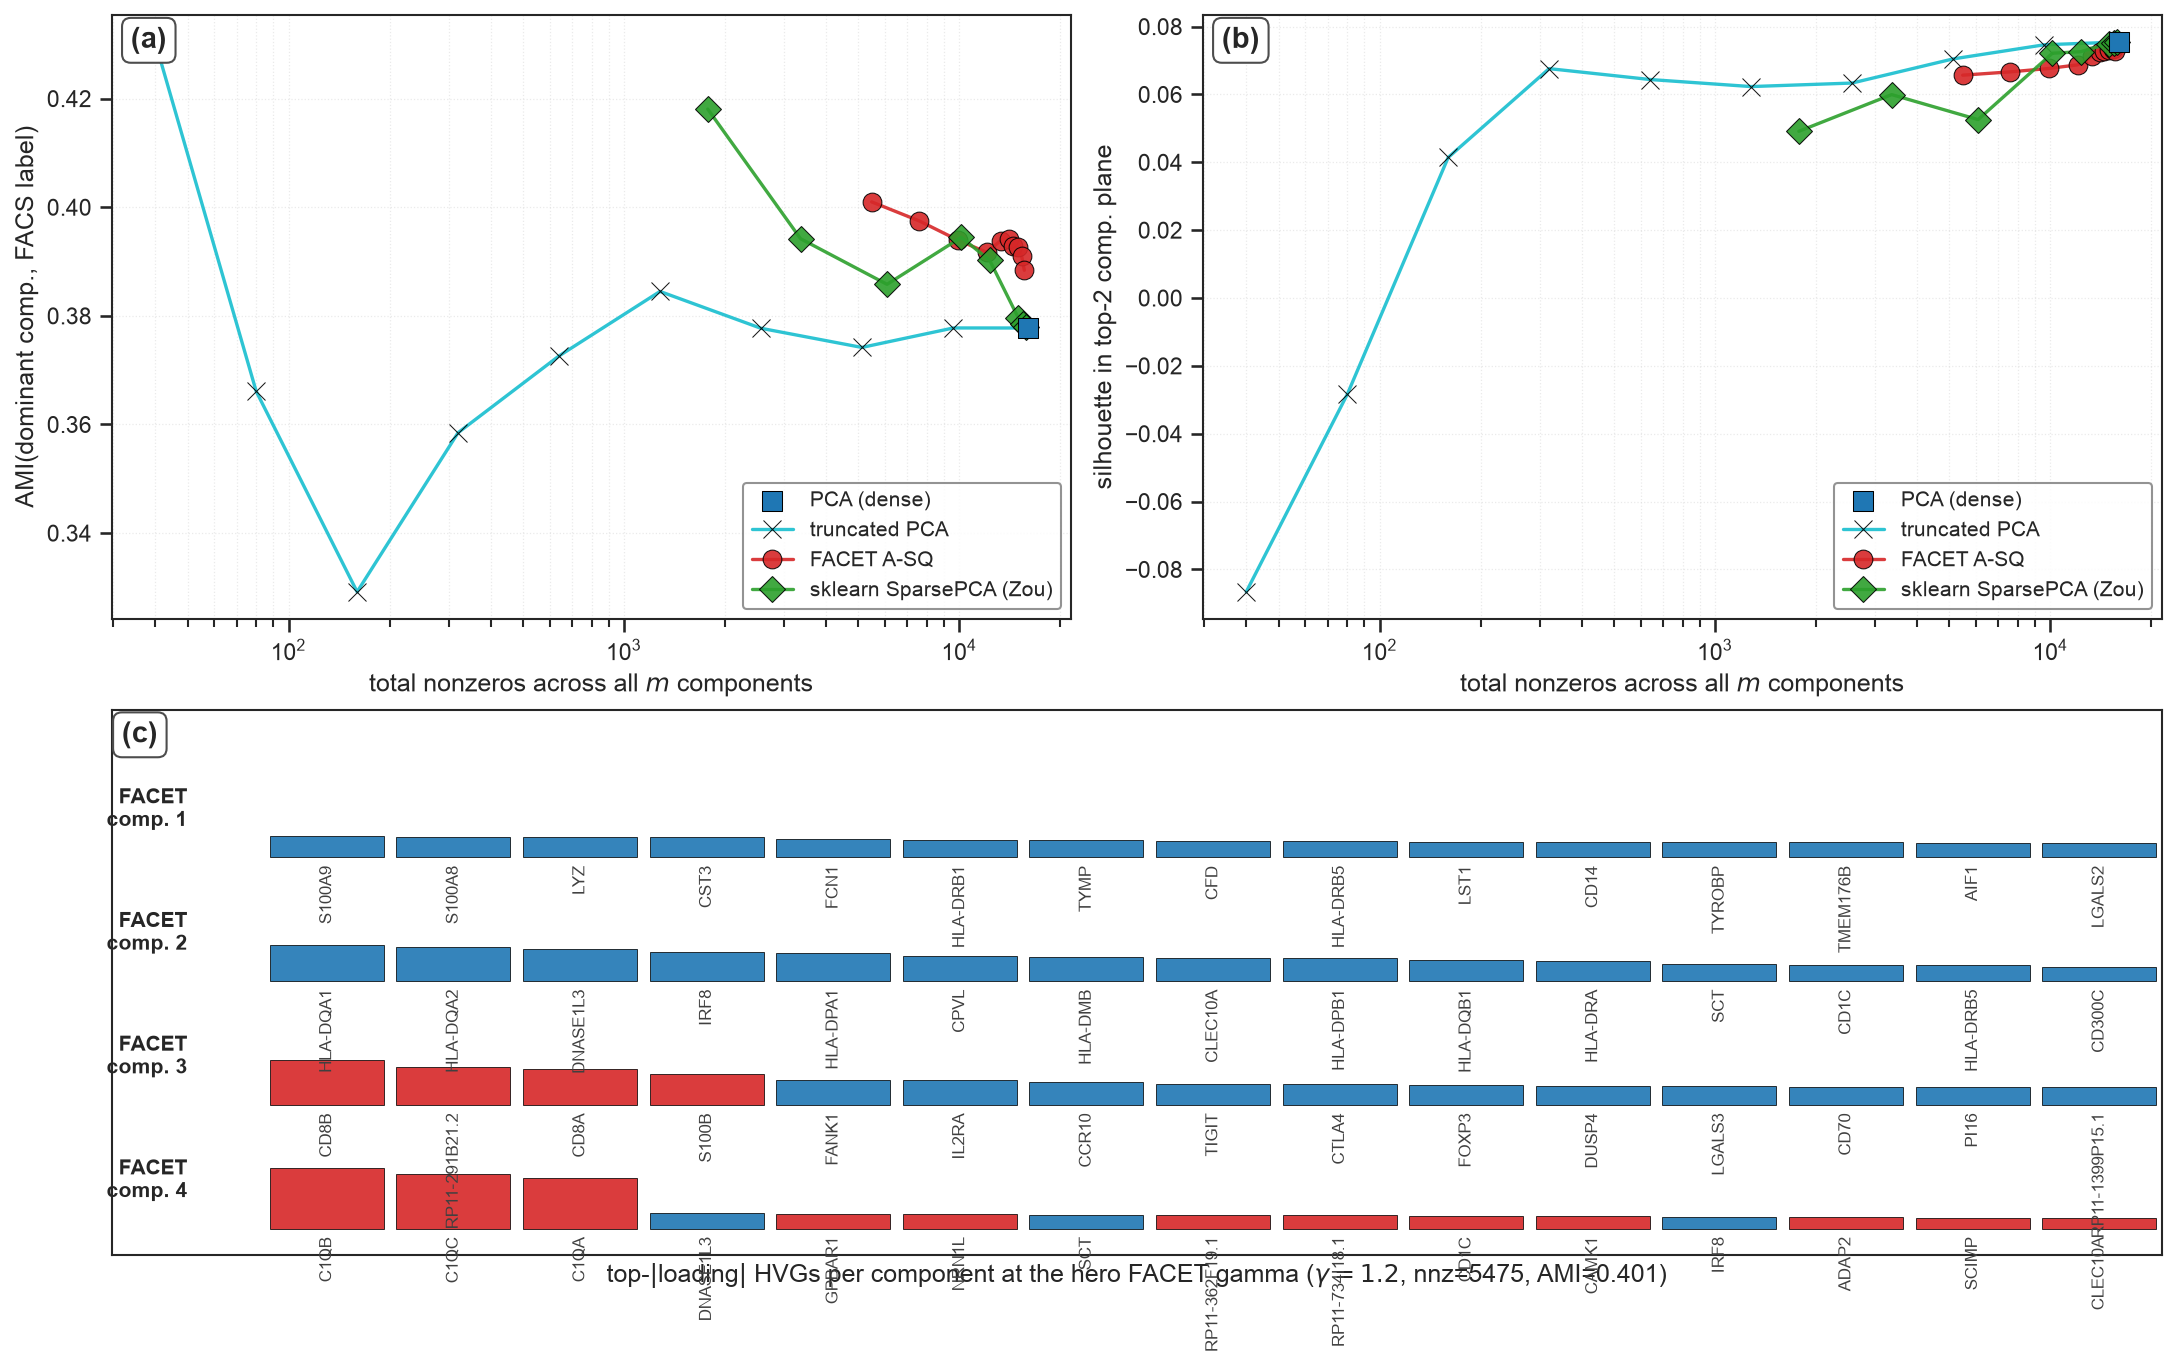
\includegraphics[width=\linewidth]{../shared/figures/generated/m9_zheng_facs_hero.png}
 \caption{\textbf{M9 Zheng17 FACS-sorted PBMCs, native cell-type labels.} Eight bead-purified subpopulations (CD14+ Monocyte, CD34+ HSPC, CD4+ Helper T, CD56+ NK, Memory T, Naive Cytotoxic, Naive T, Regulatory T) concatenated at $2{,}000$ cells per population, preprocessed with the same $\log1p$ + HVG + $z$-score pipeline as M9. Labels are the FACS gates, independent of any clustering step. \textbf{(a)}~AMI vs total nonzeros across all $m{=}8$ loadings. FACET A-SQ attains AMI $0.401$, above the dense-PCA ceiling at $0.378$, flipping the ranking seen on PCA-derived pseudo-labels in Fig.~\ref{fig:m9-scrna-hero}. \textbf{(b)}~Silhouette in the top-two component plane. \textbf{(c)}~Top-15 gene loadings per component at the hero FACET gamma.}
 \label{fig:m9-zheng-facs-hero}
\end{figure}

% Figure M9-Zheng-FACS interp hero: interpretability-first companion.
% Generated by experiments/m9_zheng_facs.py --interpretability.
\begin{figure}[t]
 \centering
 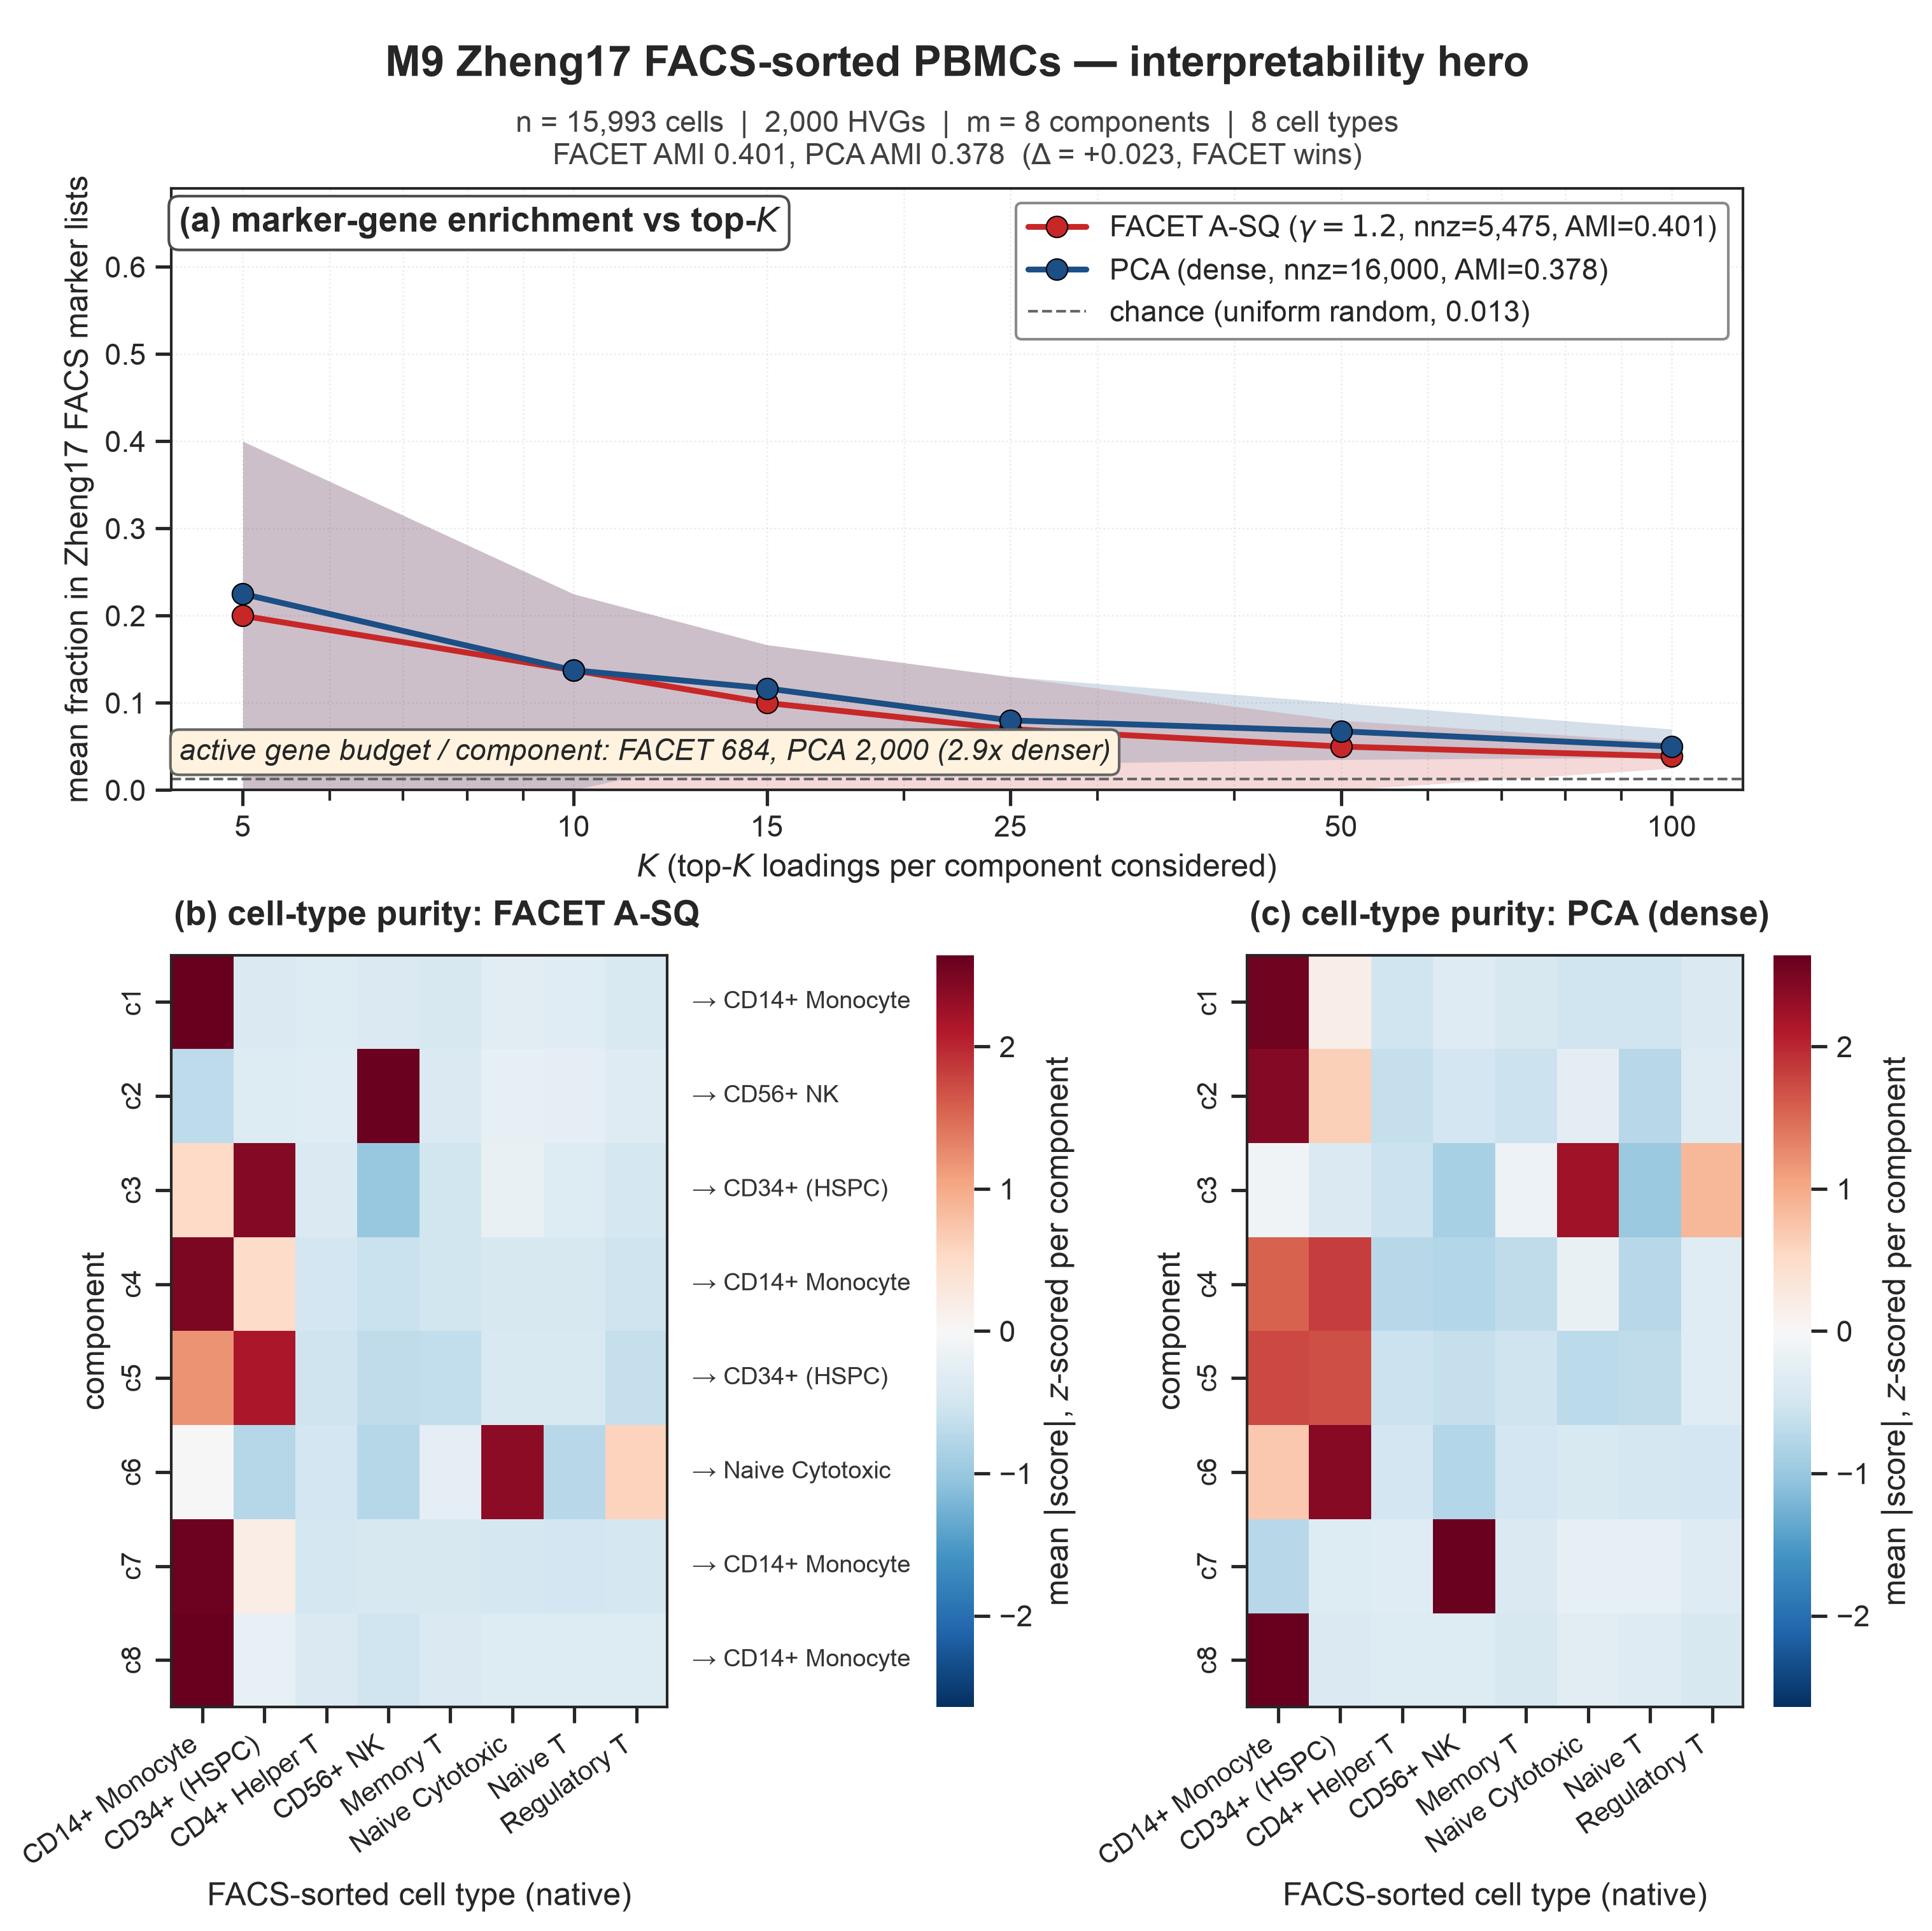
\includegraphics[width=\linewidth]{../shared/figures/generated/m9_zheng_facs_interpretability_hero.png}
 \caption{\textbf{M9 Zheng17 FACS interpretability hero.} Companion to Fig.~\ref{fig:m9-zheng-facs-hero}, interpretability-first panels on the same bead-purified data. \textbf{(a)}~Mean enrichment vs top-$K$ in the Zheng FACS marker list (CD14+ Mono, CD34+, CD4 helper, CD56+ NK, Treg, memory/naive T subsets); gene-economy banner reports the per-component active-gene budget. \textbf{(b)}~FACET cell-type purity heatmap with dominant FACS gate annotated per component (right-hand labels). Each FACET component localises on a single FACS population. \textbf{(c)}~PCA cell-type purity on the same colour scale is visibly more diffuse.}
 \label{fig:m9-zheng-facs-interp}
\end{figure}

% Figure M9-Zheng-68k hero: FACET on the 68k PBMC donor-A matrix with
% paper-published FACS-correlated per-barcode cell-type labels.
% Generated by experiments/m9_zheng68k.py --hero.
\begin{figure}[t]
 \centering
 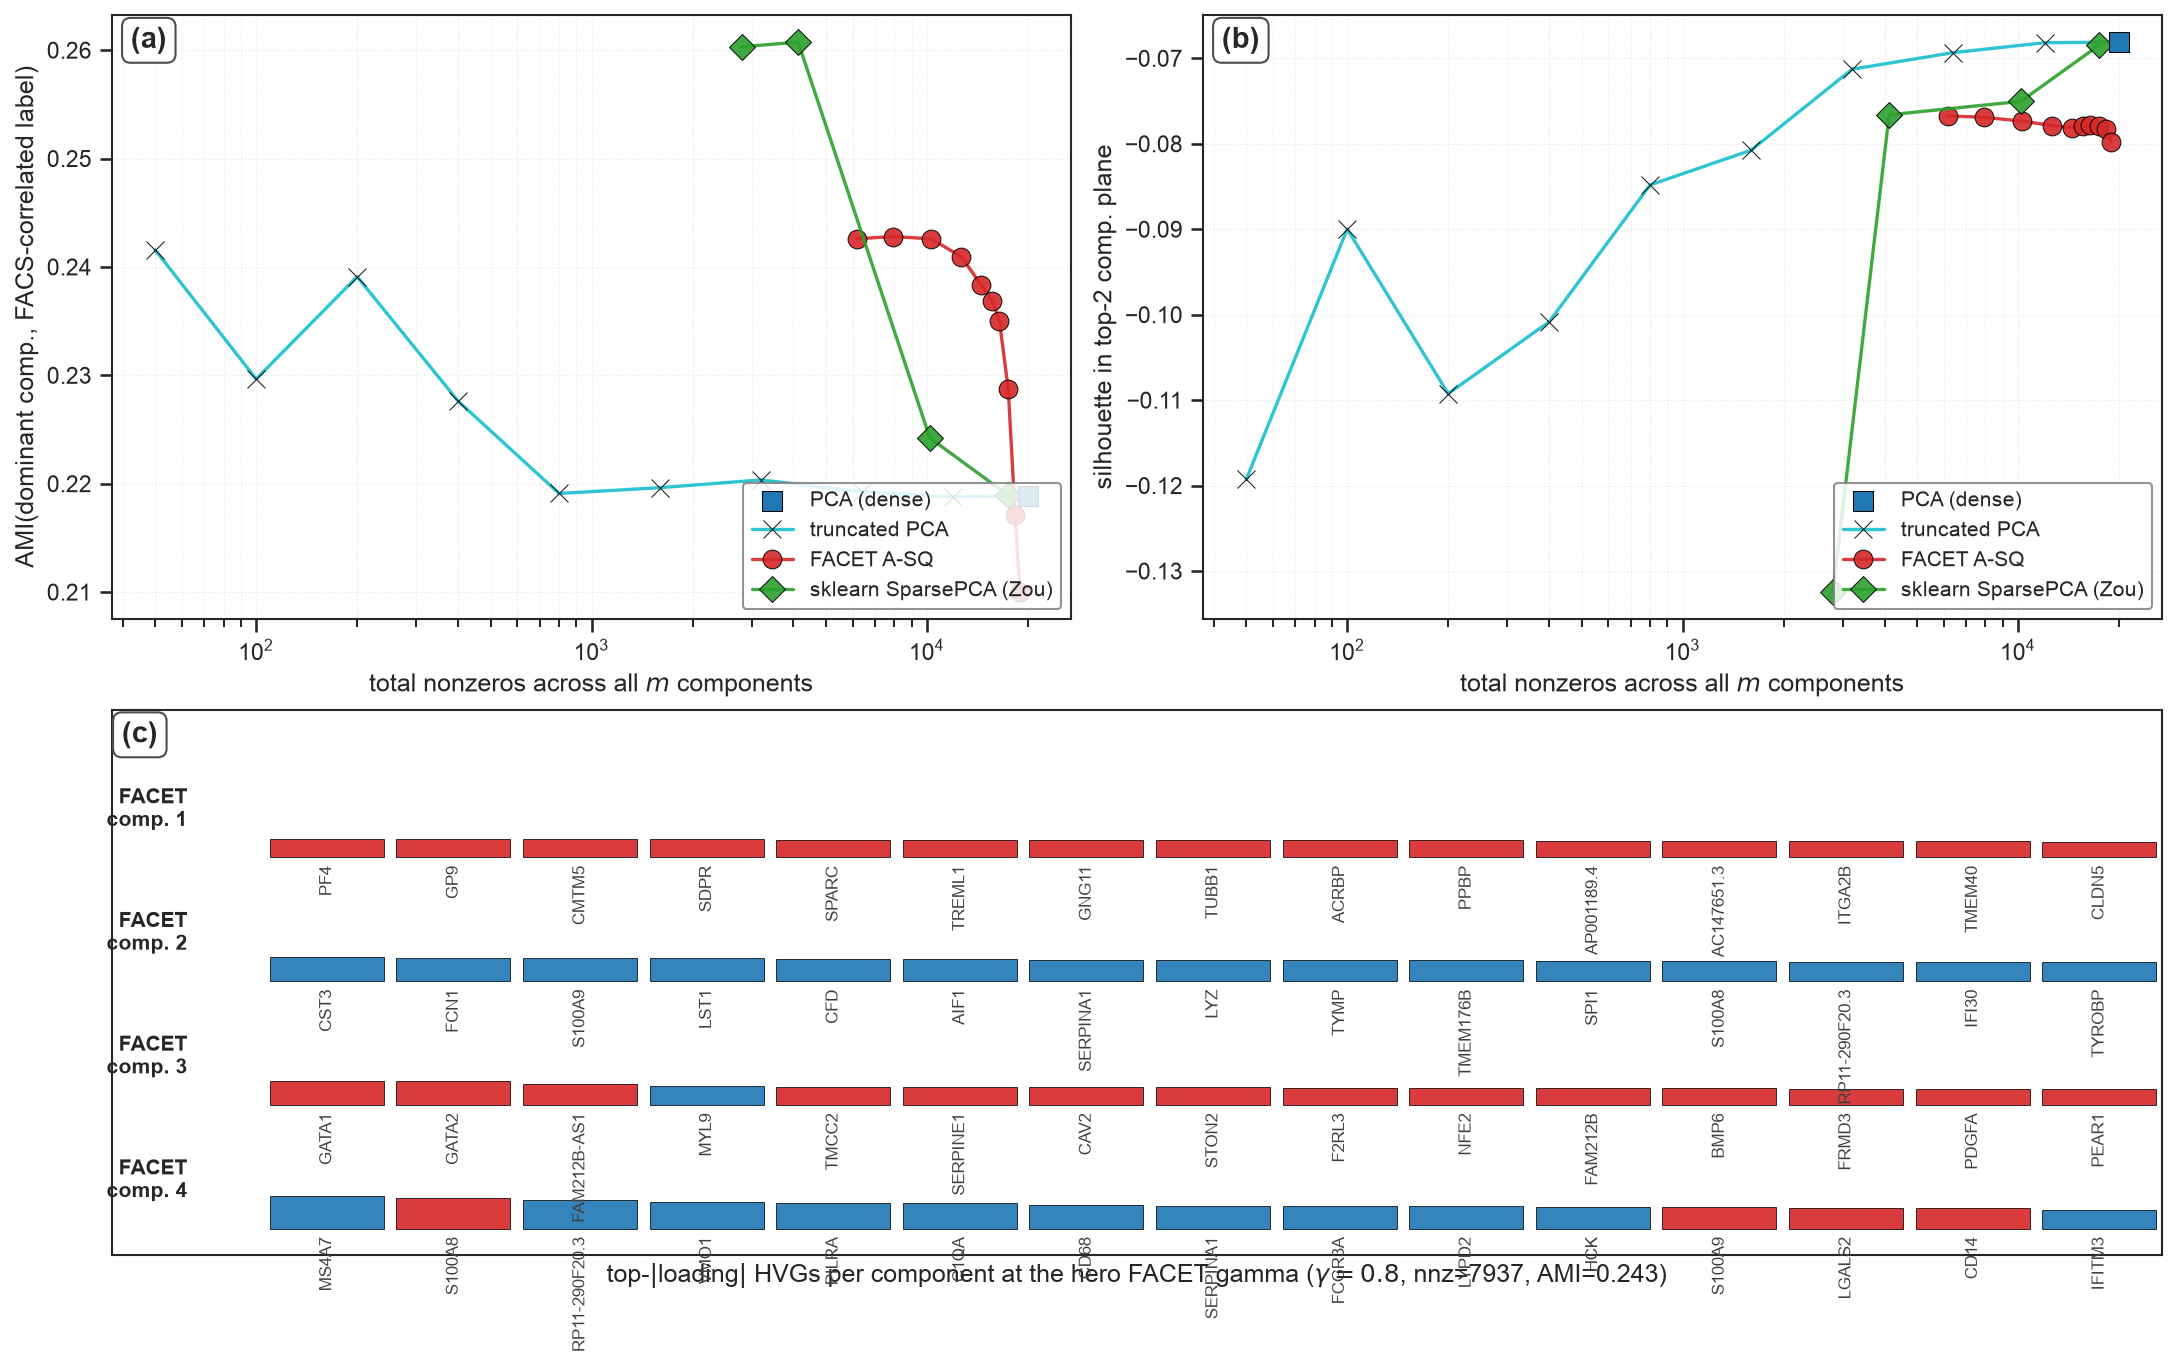
\includegraphics[width=\linewidth]{../shared/figures/generated/m9_zheng68k_hero.png}
 \caption{\textbf{M9 Zheng17 68k PBMC (donor A), native cell-type labels.} 68{,}551 cells $\times$ 2{,}000 HVGs; the per-barcode labels are the FACS-correlated cell-type assignments distributed with the Zheng et al.~2017 analysis repository, not derived from any clustering of this matrix. $m{=}10$ components. \textbf{(a)}~AMI vs total nonzeros: FACET A-SQ reaches AMI $0.243$ against the dense-PCA ceiling of $0.219$ ($+0.024$). \textbf{(b)}~Silhouette in the top-two component plane. \textbf{(c)}~Top-15 gene loadings per component at the hero FACET gamma; each component resolves into an immune programme consistent with its dominant cell type.}
 \label{fig:m9-zheng68k-hero}
\end{figure}

% Figure M9-Zheng-68k interp hero: interpretability-first companion.
% Generated by experiments/m9_zheng68k.py --interpretability.
\begin{figure}[t]
 \centering
 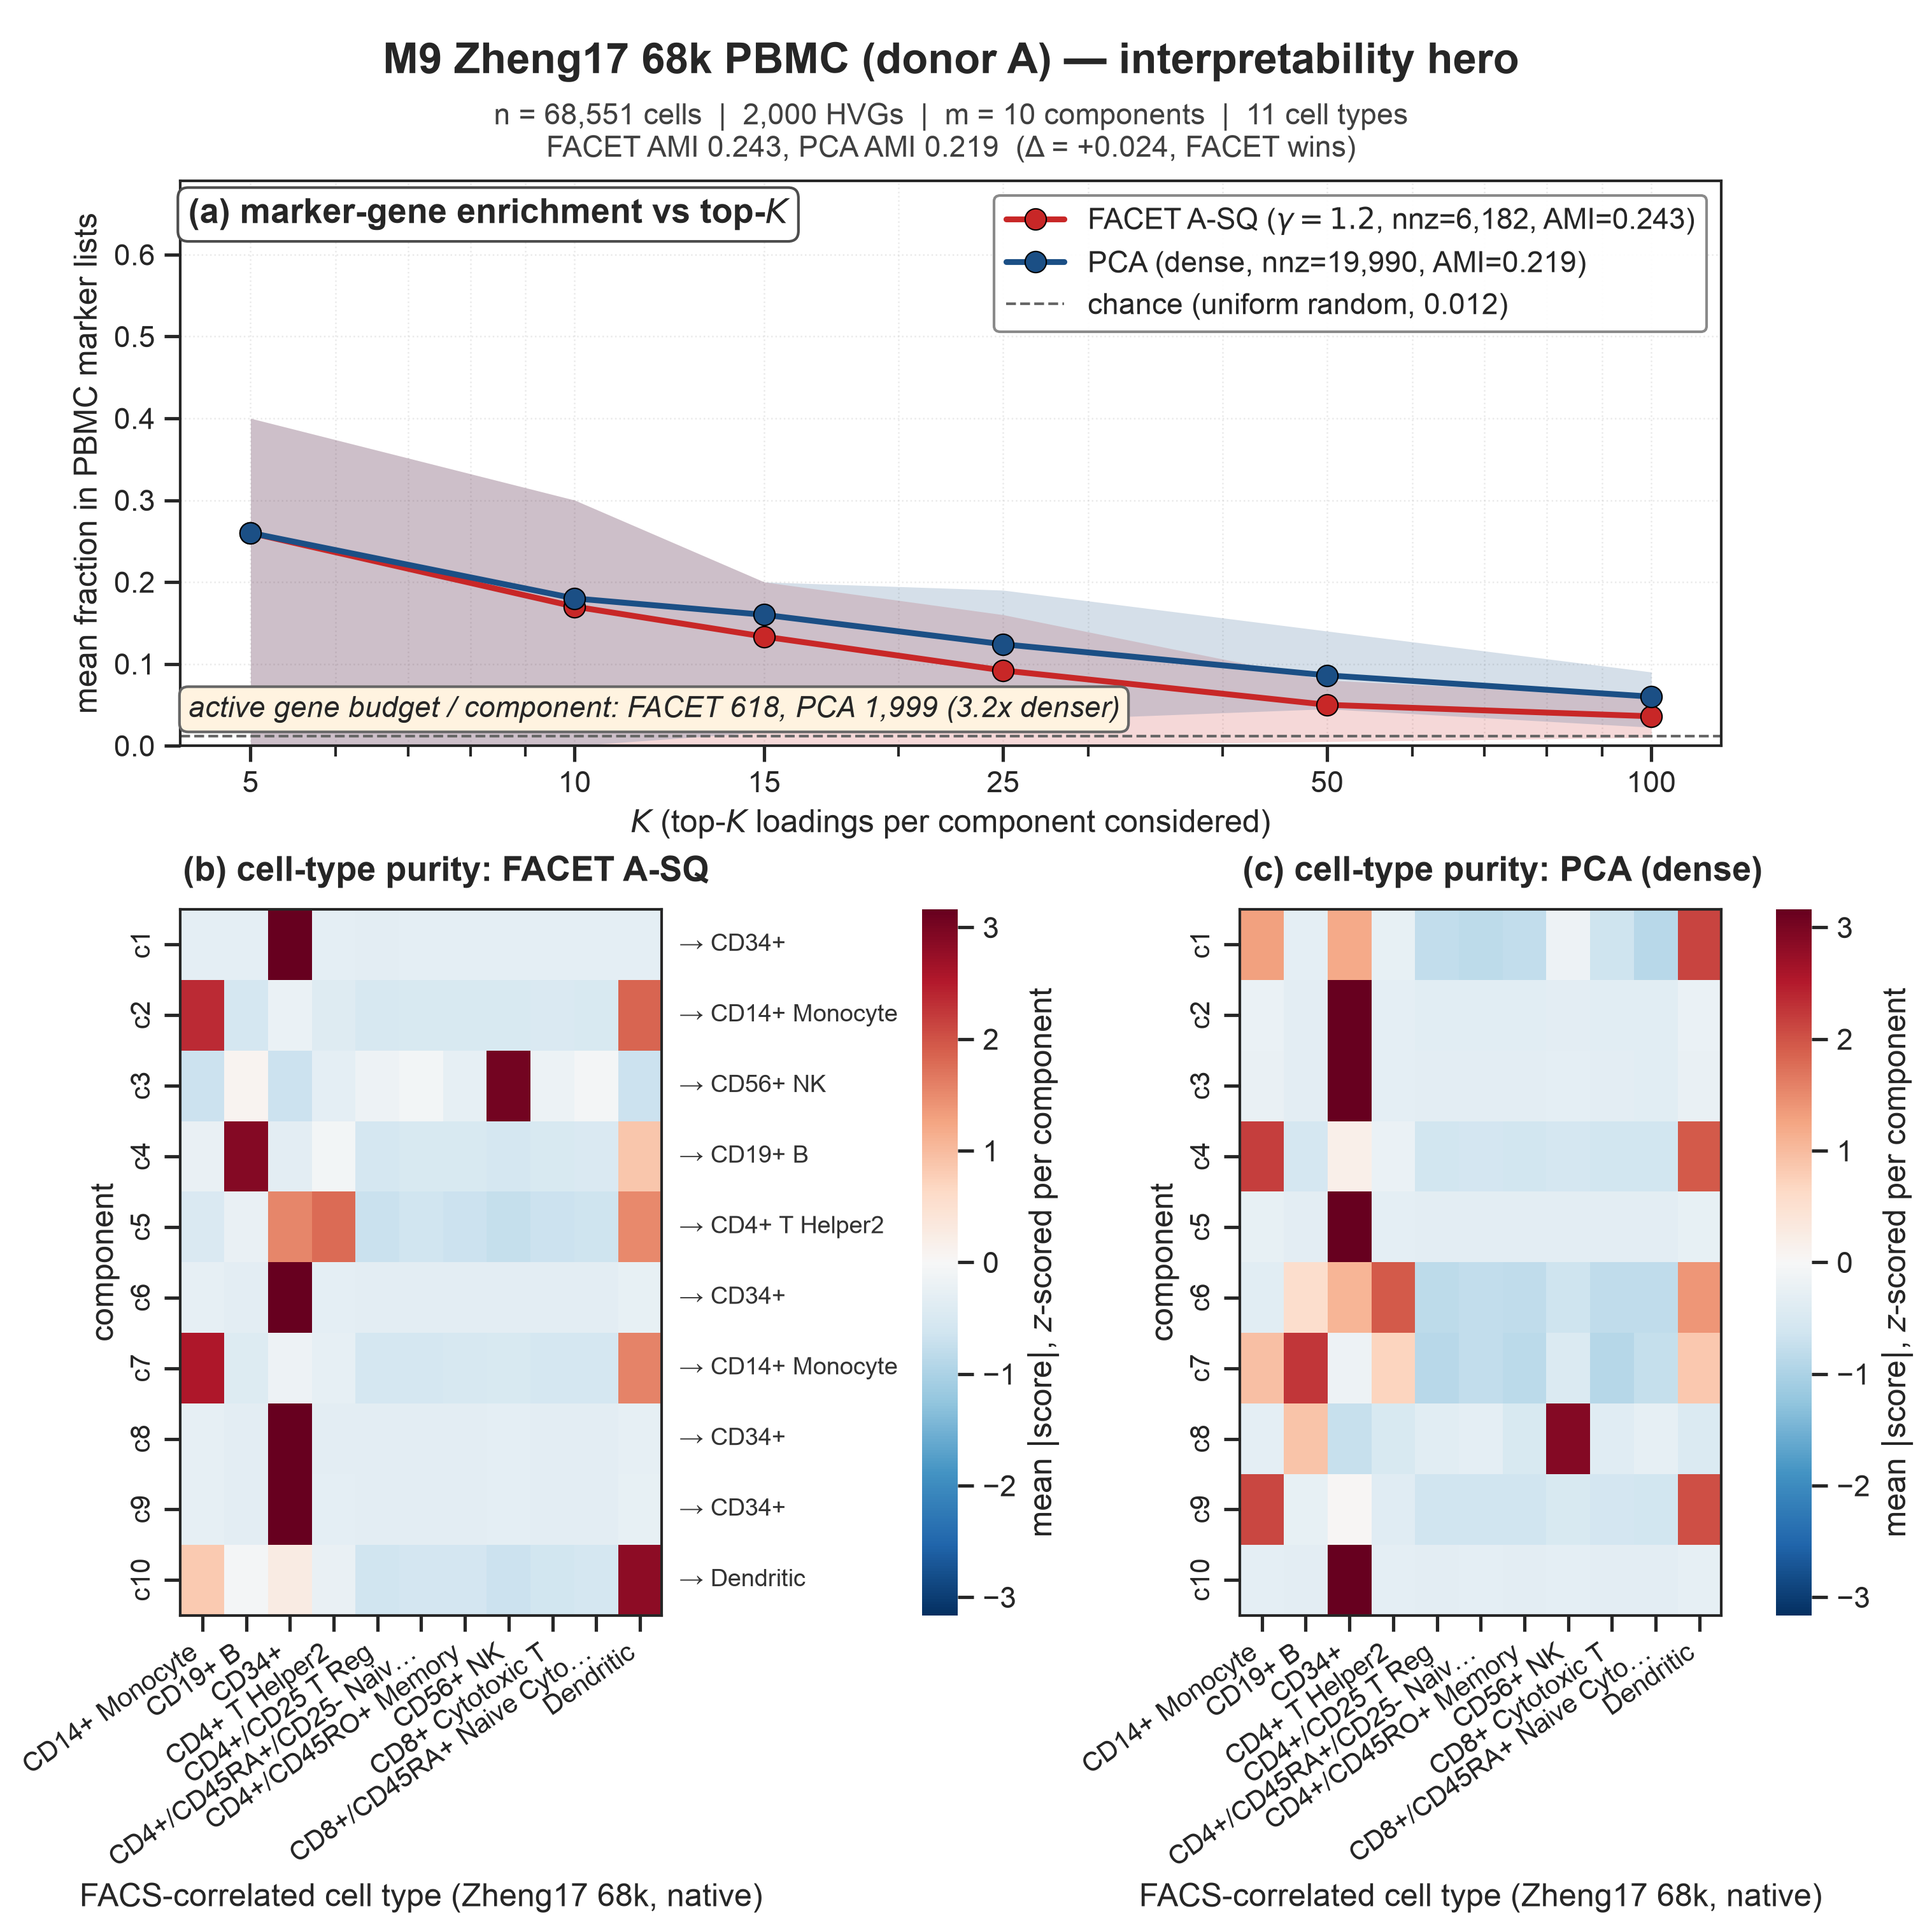
\includegraphics[width=\linewidth]{../shared/figures/generated/m9_zheng68k_interpretability_hero.png}
 \caption{\textbf{M9 Zheng17 68k interpretability hero.} Companion to Fig.~\ref{fig:m9-zheng68k-hero}. \textbf{(a)}~Mean enrichment vs top-$K$ in the PBMC marker list; the gene-economy annotation reports FACET's active-gene budget per component against PCA's. \textbf{(b)}~FACET per-component cell-type purity heatmap with the dominant FACS-correlated cell type labelled on each row. Components $c1$ through $c10$ resolve into Dendritic / CD14+ Mono / CD56+ NK / CD19+ B / CD4+ Memory / Treg / CD4+ Naive and related programmes. \textbf{(c)}~PCA purity on the same colour scale is diffuse and does not admit a clean cell-type reading per component.}
 \label{fig:m9-zheng68k-interp}
\end{figure}

% Figure M9-Tabula-Muris hero: FACET on mouse Tabula Muris FACS tissues
% (Marrow + Spleen + Thymus) with native cell_ontology_class labels.
% Generated by experiments/m9_tabula_muris.py --hero.
\begin{figure}[t]
 \centering
 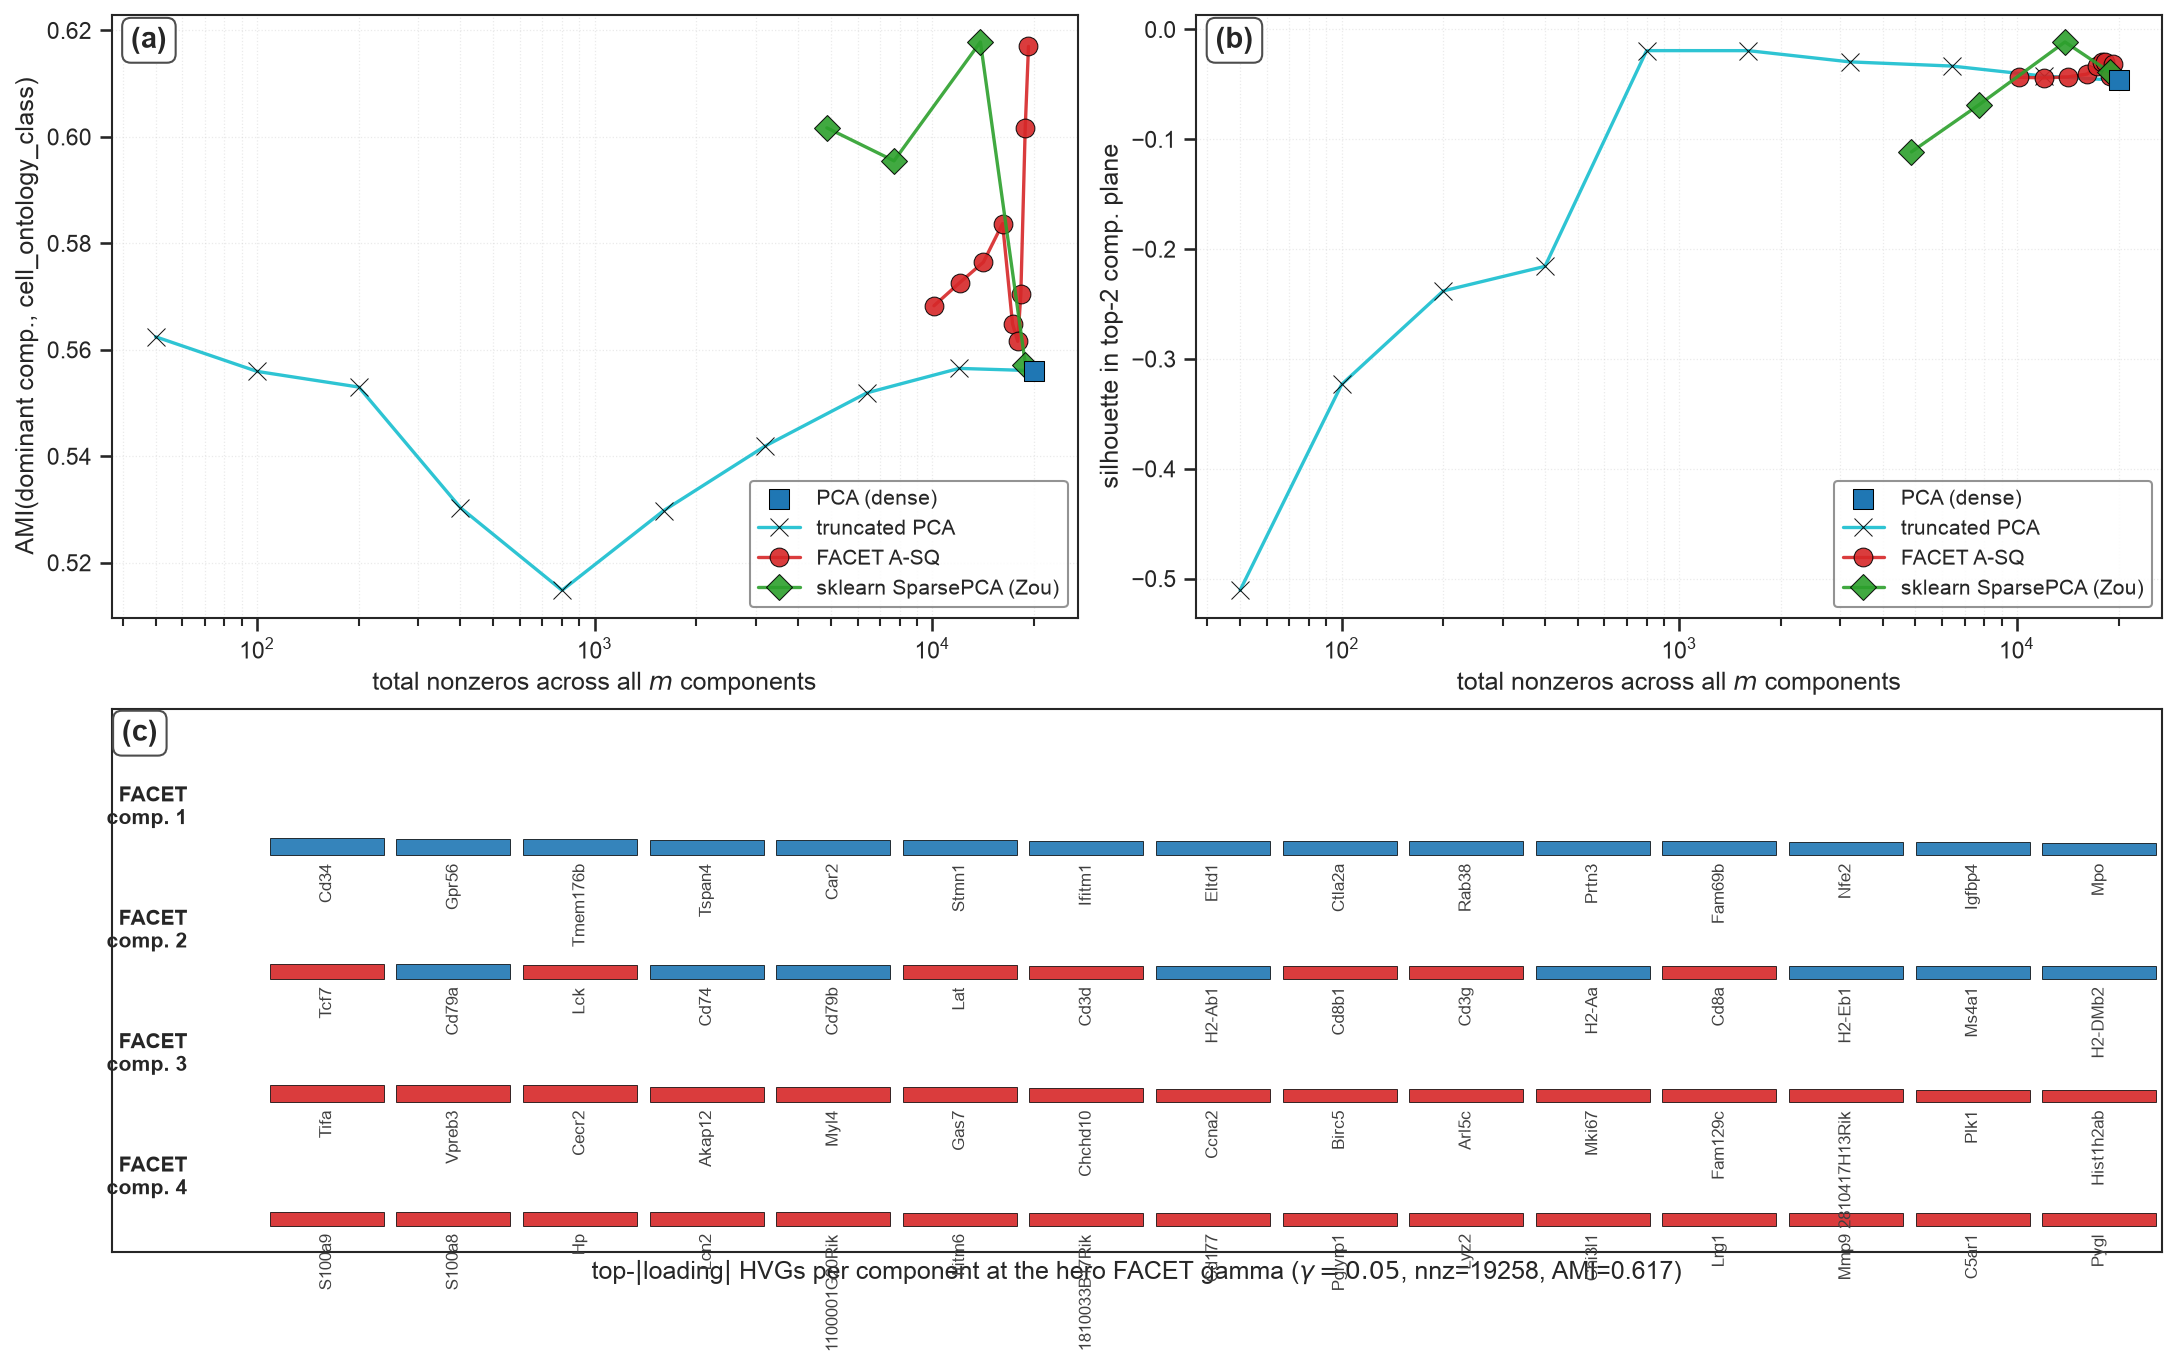
\includegraphics[width=\linewidth]{../shared/figures/generated/m9_tabula_muris_hero.png}
 \caption{\textbf{M9 Tabula Muris FACS (Marrow + Spleen + Thymus), native mouse cell-type labels.} 8{,}083 cells $\times$ 2{,}000 HVGs across $25$ \texttt{cell\_ontology\_class} categories; labels come from the official Tabula Muris annotations, not from any clustering of this matrix. $m{=}10$ components. \textbf{(a)}~AMI vs total nonzeros: FACET A-SQ reaches AMI $0.617$ against the dense-PCA ceiling of $0.556$ ($+0.061$, the largest margin of the three native-label scRNA experiments). \textbf{(b)}~Silhouette in the top-two component plane. \textbf{(c)}~Top-15 gene loadings per component at the hero FACET gamma; mouse symbols (title-case).}
 \label{fig:m9-tabula-muris-hero}
\end{figure}

% Figure M9-Tabula-Muris interp hero: interpretability-first companion.
% Generated by experiments/m9_tabula_muris.py --interpretability.
\begin{figure}[t]
 \centering
 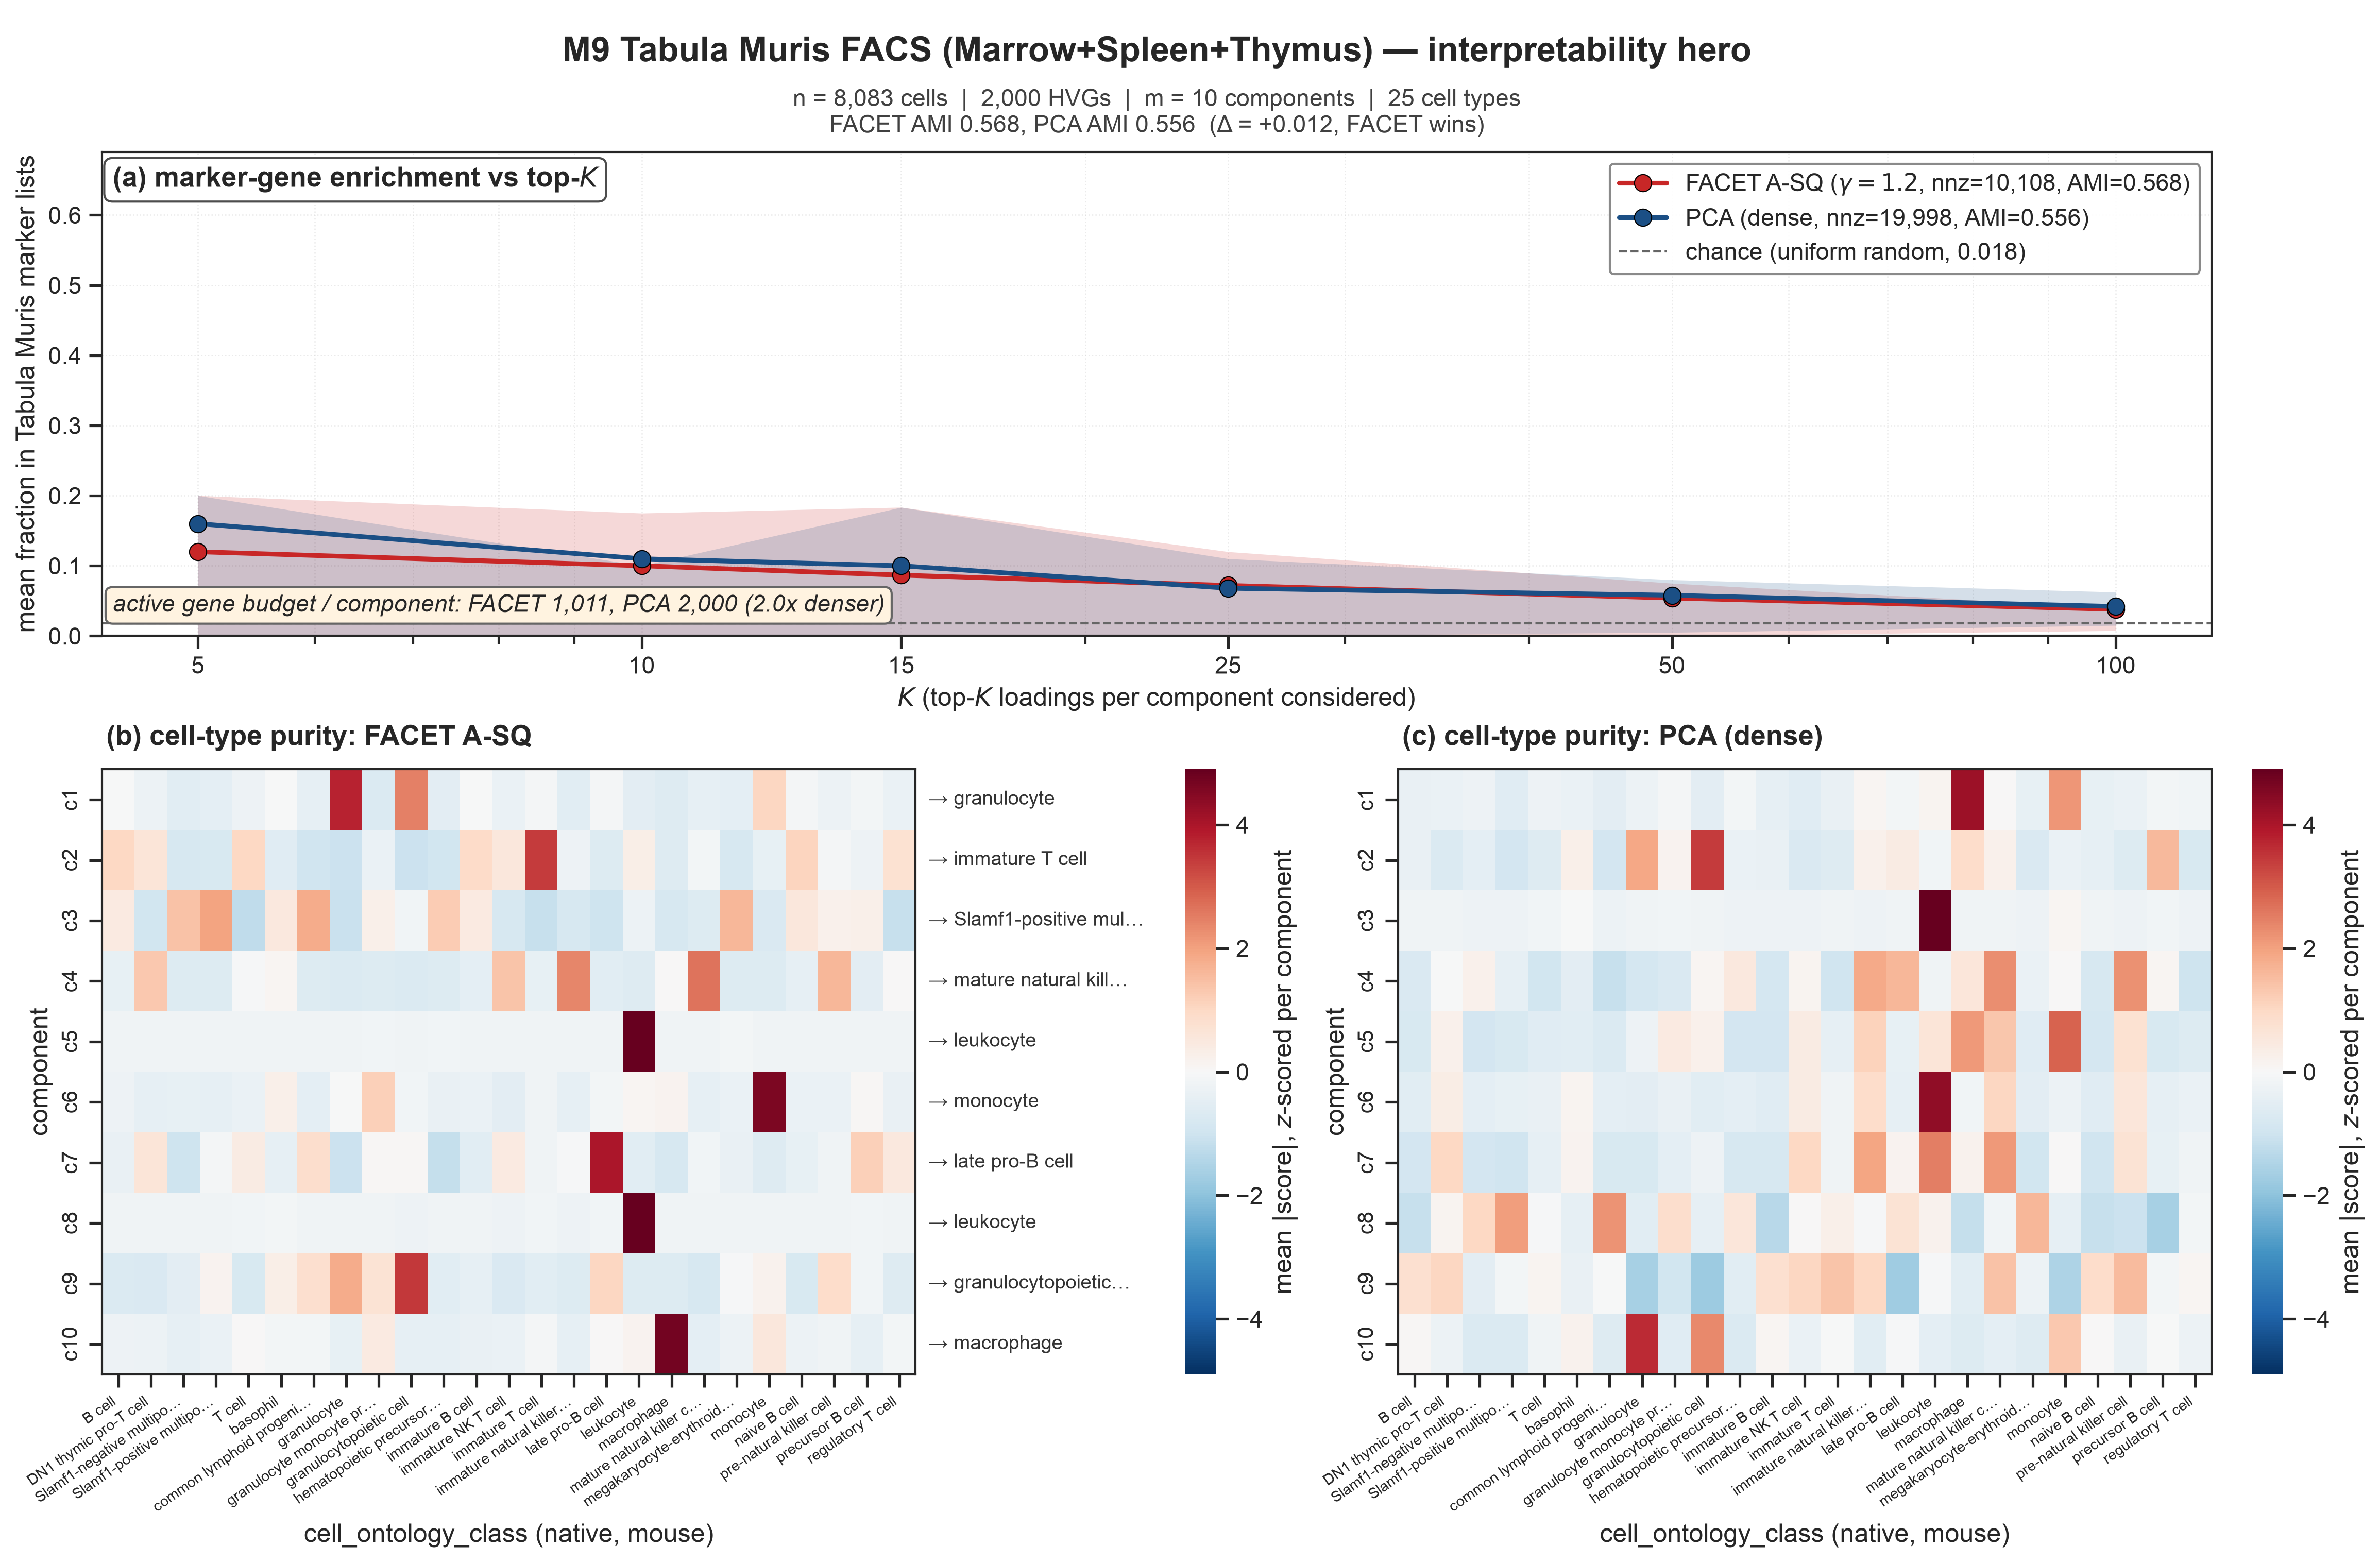
\includegraphics[width=\linewidth]{../shared/figures/generated/m9_tabula_muris_interpretability_hero.png}
 \caption{\textbf{M9 Tabula Muris interpretability hero.} Companion to Fig.~\ref{fig:m9-tabula-muris-hero}, interpretability-first panels on the same mouse Smart-seq2 data. \textbf{(a)}~Mean enrichment vs top-$K$ in the mouse immune / stromal marker list; gene-economy annotation reports per-method active-gene budget per component. \textbf{(b)}~FACET cell-type purity heatmap with dominant \texttt{cell\_ontology\_class} annotated per row. \textbf{(c)}~PCA cell-type purity on the same colour scale.}
 \label{fig:m9-tabula-muris-interp}
\end{figure}

% Figure M10 hero prototype : generated by experiments/m10_agentic.py --hero.
% Preview-only; not yet linked from the main manuscript.
\begin{figure}[t]
 \centering
 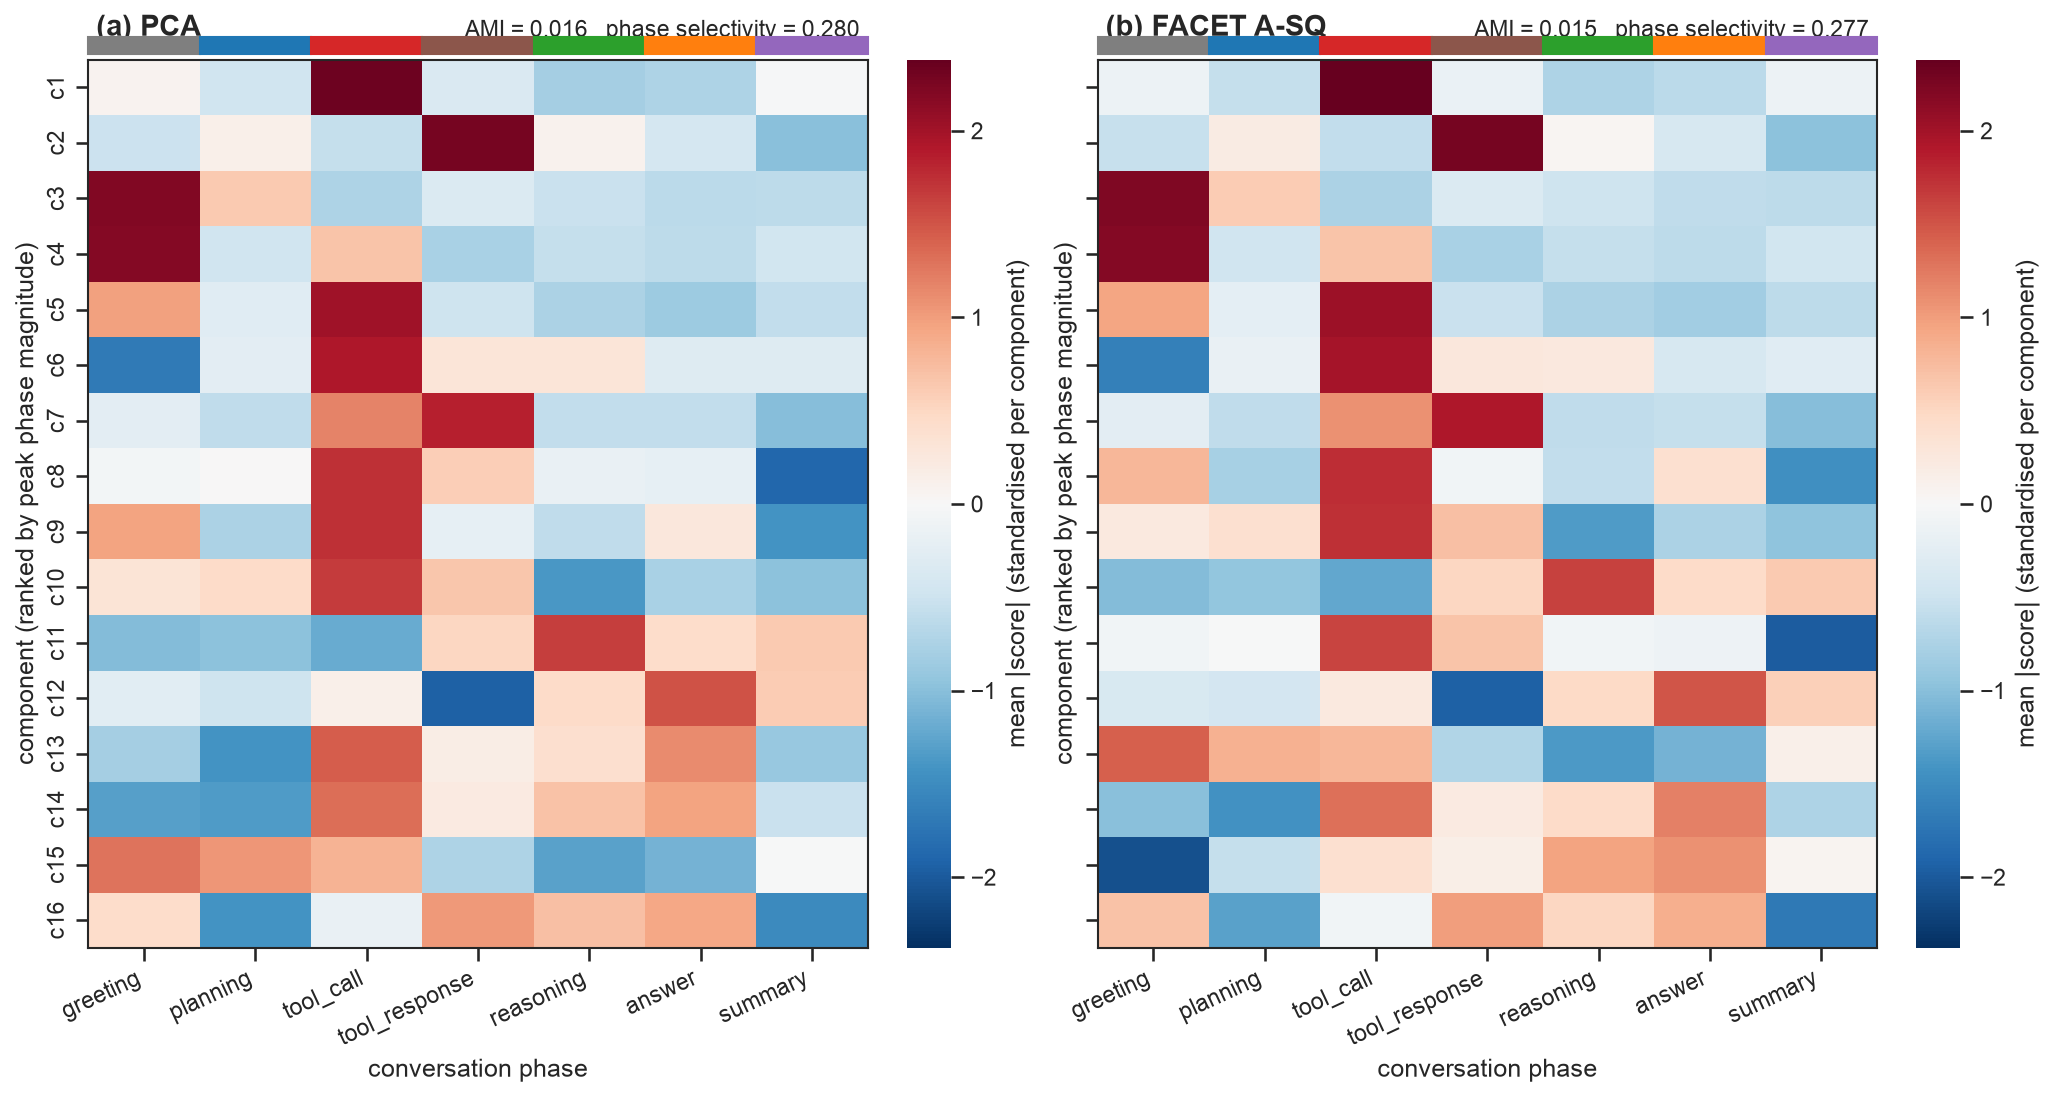
\includegraphics[width=\linewidth]{../shared/figures/generated/m10_agentic_hero.png}
 \caption{\textbf{M10: agentic AI, component--phase heatmap on multi-turn tool-use conversations.} Seven hand-written conversations alternate through \texttt{greeting}, \texttt{planning}, \texttt{tool\_call}, \texttt{tool\_response}, \texttt{reasoning}, \texttt{answer}, and \texttt{summary} phases ($836$ tokens total). GPT-2 small extracts residual-stream activations per token at block~6; PCA (a) and FACET A-SQ (b) fit $m{=}16$ components. Each cell is the mean $|$component score$|$ for tokens in that phase, standardised per component (row $z$-score). Rows are sorted by peak phase magnitude. The in-panel badges report the dominant-component AMI against the ground-truth phase label and the mean per-component ``phase selectivity'' $(\max - \mathrm{median})/\max$. FACET components concentrate activity on \texttt{tool\_call}, \texttt{tool\_response}, and \texttt{greeting} spikes (red/blue bands) while PCA spreads activity more uniformly across phases.}
 \label{fig:m10-agentic-hero}
\end{figure}


\subsection{Qualitative pattern (observed)}
The panels confirm the predicted qualitative pattern. Larger strict margins produce earlier support identification (Q3). In the fixed-support hard-threshold regime, the active eigengap predicts the observed angle-contraction slope to within $5\%$ when $\gamma{=}0$ (Q4, panel a); the soft-threshold branch tracks the corrected prediction $\lambda_2 / (\lambda_1 - \gamma\,\sigma_1\sqrt{k})$ to within $1\%$ (Q4, panel b). A-SUM and A-SQ diverge most when component response energies are heterogeneous (Q1 counterexample). Restricted refitting dominates raw selection on every point (A4). Safe screening gives its full $(n-k)/n$ oracle-work saving once the certified basin is entered, with zero objective loss (M7).

\subsection{Analysis order}
The analysis proceeds from formulation checks (Q1), through margin and rate diagnostics (Q2, Q3, Q4, A4), through the controlled-neural bridge (T2), to real open-model activations (T3 and the M-panels). For each result, the panel caption states the relevant assumption diagnostic next to the empirical metric. Downstream gains after recalibration or fine-tuning are not credited to support selection without matched-support controls.

\subsection{Negative evidence}
Threshold cycling at zero margin, sensitivity to rank-deficient polar completions, and noncontractive heterogeneous-support fixed points are scientifically informative. They determine the scope of the final theorem and remain in the manuscript rather than being removed as implementation failures.
